\chapter{\protect Results and Discussions}
\label{results}
According to the New Horizons team \cite{Grundy2016formation}, CH$_4$ from Pluto may accumulate by cold-trapping, onto surface of Charon. The amount of CH$_4$ varies throughout the surface of Charon because it depends on duration of temperature below 25 K. The duration depends on diurnal motion and thermal inertia of Charon. With a tilted axis of 112 degrees to the ecliptic, higher concentration of CH$_4$ will accumulate at the pole (see chapter \ref{introduction} for details). Therefore, we investigate different concentrations of CH$_4$+NH$_3$ ice mixtures and answer several questions: Will different concentration of CH$_4$ mix with high concentration of ammonia observed on crater position and throughout the surface of Charon \cite(Grundy2016formation) have structure difference in accumulation of tholin? Are there variations of photo-products when concentration of CH$_4$ differ during warm-up? Since both EUV and VUV irradiation irradiates onto Charon, are there any differences when we change the photon source from VUV to EUV to irradiate the ice mixtures?\\

The main source to irradiate the dark side of Charon is Lyα reflected by interplanetary medium \cite{Grundy2016formation}. Other sources such as the energetic ions in solar wind, consists of mainly H$^+$, He$^+$, He$^{++}$ and O$^{2+}$ etc are originated from solar corona or IPM. These ions would also reflect solar irradiation to the dark side of Charon. Among these irradiations, we picked He II irradiation because He II is 3 – 20 times more intense then He I during a solar flare. As it varies, it is difficult to estimate the dose onto Charon. Besides, electronic flux is also present in solar wind but it is one order of magnitude lower than proton flux. The flux for energetic electrons observed at the 1 A. U. position is available (http://www.swpc.noaa.gov/products/goes-electron-flux). Although electron flux is much less important than Lyα, and their flux varies, we also compare the electron irradiation experiment done by Kim and Kaiser \cite{kim} on CH$_4$+NH$_3$ ice mixtures.\\

When Charon is shine by direct sun light, the surface temperature increases and deliver the heat to the poles by conduction. From the model of Grundy \cite{Grundy2016formation}, the surface temperature of the pole area would increase to 60 K that the heating rate depends on the thermal conductivity of Charon. To demonstrate the heating process, we warmup our ice mixture with a heating rate 1 K/min and monitor the ice by both QMS and scanning IR spectra with 5 K intervals. We will look into whether there are new species formed during warmup and monitor the gas phase desorption.\\

Finally, after we focus on the concentration effect of CH$_4$ on photo-products, photon energy effects, species detected during warmup phases, we present the residues accumulated by irradiating CH$_4$+NH$_3$ ice mixtures with different ratios. Since both tholin formed on Titan and Charon has similar colour, we also compare the IR spectra of MDHL, NSRRC with different configurations with the residues on Titan with experiments done by Imanaka et al. \cite{imanaka2004laboratory}\\
\section{The infra-red spectrums and peaks identification}
Before and after deposition, we scanned an IR spectrum and plotted the absorbance of the ice mixtures. Figure \ref{fig:widerange} is a plot of the absorbance of the CH$_4$+NH$_3$ ice mixtures in different ratios of CH$_4$+NH$_3$ ice mixtures, from top to bottom 1:20, 1:10, 1:5 and 3:2. We have labelled the peaks which we used to calculate the column densitiesby dotted lines throughout the graph. Main products we have detected are C$_2$H$_6$, CN$^-$ and C$_3$H$_8$. The peak positions with the references are listed in Table \ref{tab:WavenumberMDHL}.\\

\begin{figure}
\centering
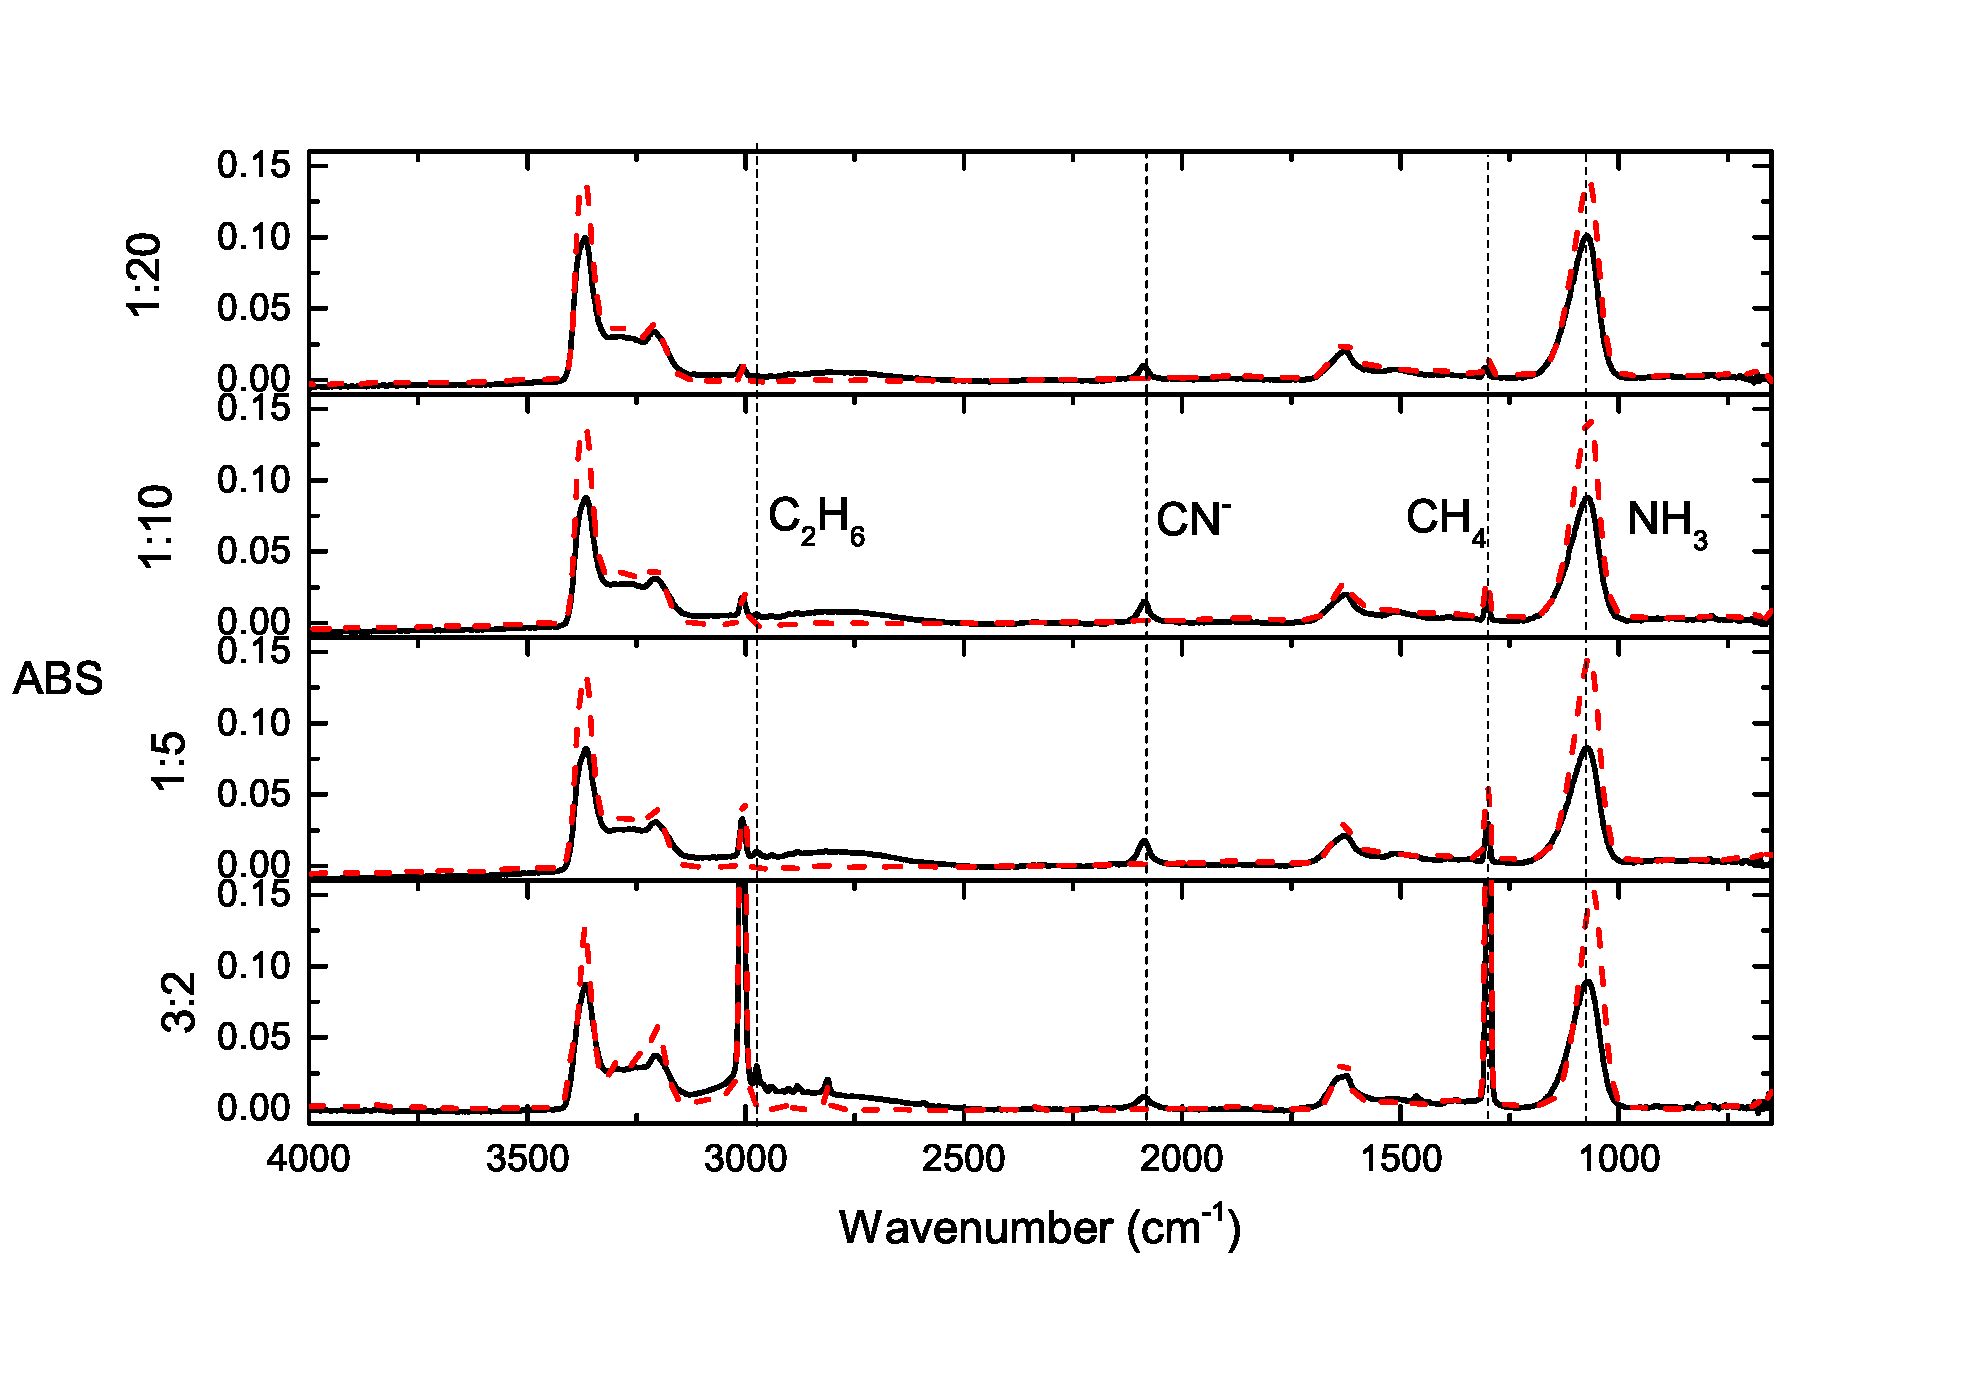
\includegraphics[width=\textwidth]{figures/chapter3/widerange.eps}
\caption{The the infra-red spectrum of CH$_4$ + NH$_3$ ice mixtures before irradiation (dashed) and VUV irradiated ice mixtures provided by MDHL. }
\label{fig:widerange}
\end{figure}

\begin{table}[htbp]
\caption{The peak positions of identified substances after irradiation in different configurations of ice mixtures.}
\label{tab:WavenumberMDHL}
\begin{tabular}{ccccccc}
\hline
\hline
\multicolumn{2}{c}{Literture assignments} & \multicolumn{4}{c}{CH$_4$+NH$_3$ ratio (MDHL)} &  \\
\hline
Wavenumber & Carrier  & 1:5  & 1:10  & 1:20  & 3:2  & Ref. \\
(cm$^{-1}$) &   & (cm$^{-1}$) & (cm$^{-1}$) & (cm$^{-1}$) & (cm$^{-1}$) &\\
\hline
3375 & $\nu_3$ (NH$_3$) & 3366 & 3366 & 3369 & 3367 & 1 \\
3290 & $2\nu_4$ (NH$_3$) & - & - & - & - & 1 \\
3210 & $\nu_1$ (NH$_3$) & 3207 & 3208 & 3210 & 3205 & 1 \\
3011 & $\nu_3$ (CH$_4$) & - & - & - & - & 2 \\
2972 & $\nu_{10}$ (C$_2$H$_6$) & 2975 & - & - & 2975 & 3 \\
2960 & C$_3$H$_8$ & - & - & - & 2960 & 7 \\
2941 & $\nu_8+\nu_11$ (C$_2$H$_6$) & 2940 & - & - & 2940 & 3 \\
2904 & $\nu_1$ (CH$_4$) & 2901 & - & - & 2901 & 5 \\
2879 & $\nu_5$ (C$_2$H$_6$) & 2882 & 2883 & - & 2882 & 3 \\
2814 & $\nu_2+\nu_4$ (CH$_4$) & - & - & - & 2815 & 5 \\
2083 & $\nu$ (CN$^-$) & 2088 & 2087 & 2088 & 2088 & 2 \\
1625 & $\nu_4$ (NH$_3$) & 1625 & 1625 & 1626 & 1631 & 1 \\
1514 & $\delta$ (NH$_2$) & 1509 & 1507 & 1505 & 1511 & 6 \\
1465-1440 & deform CH$_2$ scissor & 1461 & - & - & 1463 & 3,4 \\
1390-1370 & CH$_3$ sym deform & 1394 & 1394 & 1394 & 1372 & 4 \\
1298 & $\nu_4$ (CH$_4$) & 1301 & 1302 & 1305 & 1299 & 2 \\
1075 & $\nu_2$ (NH$_3$) & 1073 & 1072 & 1072 & 1072 & 1 \\
820 & $\nu_12$ (C$_2$H$_6$) & - & - & - & 820 & 3 \\
\hline
\end{tabular}\\
Reference: 1. Bossa et al 2008 2. Moore and Hudson 2003 3. Kim et al. 2010 4. Socrates 2001 5. Bennet and Kaiser 2007 6. Zheng et al. 2008 7. Hudson and Moore 2004
\end{table}


We integrated the area and divided by the absorption strength stated in table 3.2. Although we understand that there is an average error in absorption strengths of no more than 10 \%  when the pure ice is diluted in N$_2$ and H$_2$O \cite{richey2012near}. In our case, absorption strengths changes after CH$_4$ and NH$_3$ are mixed. For example, according to d' Hendecourt and Allamandola \cite{d1986time}, the band of NH$_3$ located at 1070 cm$^{-1}$ would not change much (from $1.1 \times 10^{-17}$ to $1.2 \times 10^{-17}$) when excess water is added to pure NH$_3$ and therefore, we may use the same absorption strength throughout our discussion to give a brief concept on what is the column density of the species and how is the absorption area changes when concentrations of ice mixtures and photon energy are changed. For the case of CN$^-$, we know that CN$^-$ has a bond order =3 by its molecular orbitals which is different from CN stretching (bond order 2.5) which is very sensitive to the matrix environment. As an example, by Borget et al. \cite{borget2012aminoacetonitrile}, the CN stretch in amino acetonitrile change by factor of 2 between the pure molecule itself and in a mixture of amino acetonitrile and H$_2$O (1:3). Here, we adopt the absorption strengths stated in Table \ref{tab:Absorbance} and neglect the error in absorption strengths.\\

\begin{table}[htbp]
\caption{The strength of absorbance adopted in this thesis measured in literatures of pure ice samples}
\label{tab:Absorbance}
\begin{tabular}{cccccc}
\hline
\hline
Wavenumber (cm$^{-1}$) & Assignment  & Vibration & FWHM & A value ($\times 10^{-17}$) & Reference \\
\hline
2976 &  C$_2$H$_6$ & -CH$_3$ & - & 1.05 & 2 \\
2960 & C$_3$H$_8$ & -CH$_2$- & - & 2.58 & 2 \\
2086 & CN$^-$ & CN & - & 1.8 & 3 \\
1297 & CH$_4$ & CH deformation & 8 & 0.61 & 1 \\
1070 & NH$_3$ & "umbrella mode" & 68 & 1.7 & 1 \\
\hline
\end{tabular}
Reference: 1. d'Hendecourt and Allamandola (1986)\cite{d1986time} 2. Moore and Hudson (1998)\cite{moore1998infrared} 3. Noble et al. (2013) \cite{noble2012thermal}
\end{table}

\section{Reaction mechanisms}

\subsection{C$_2$H$_6$}

\begin{figure}
\centering
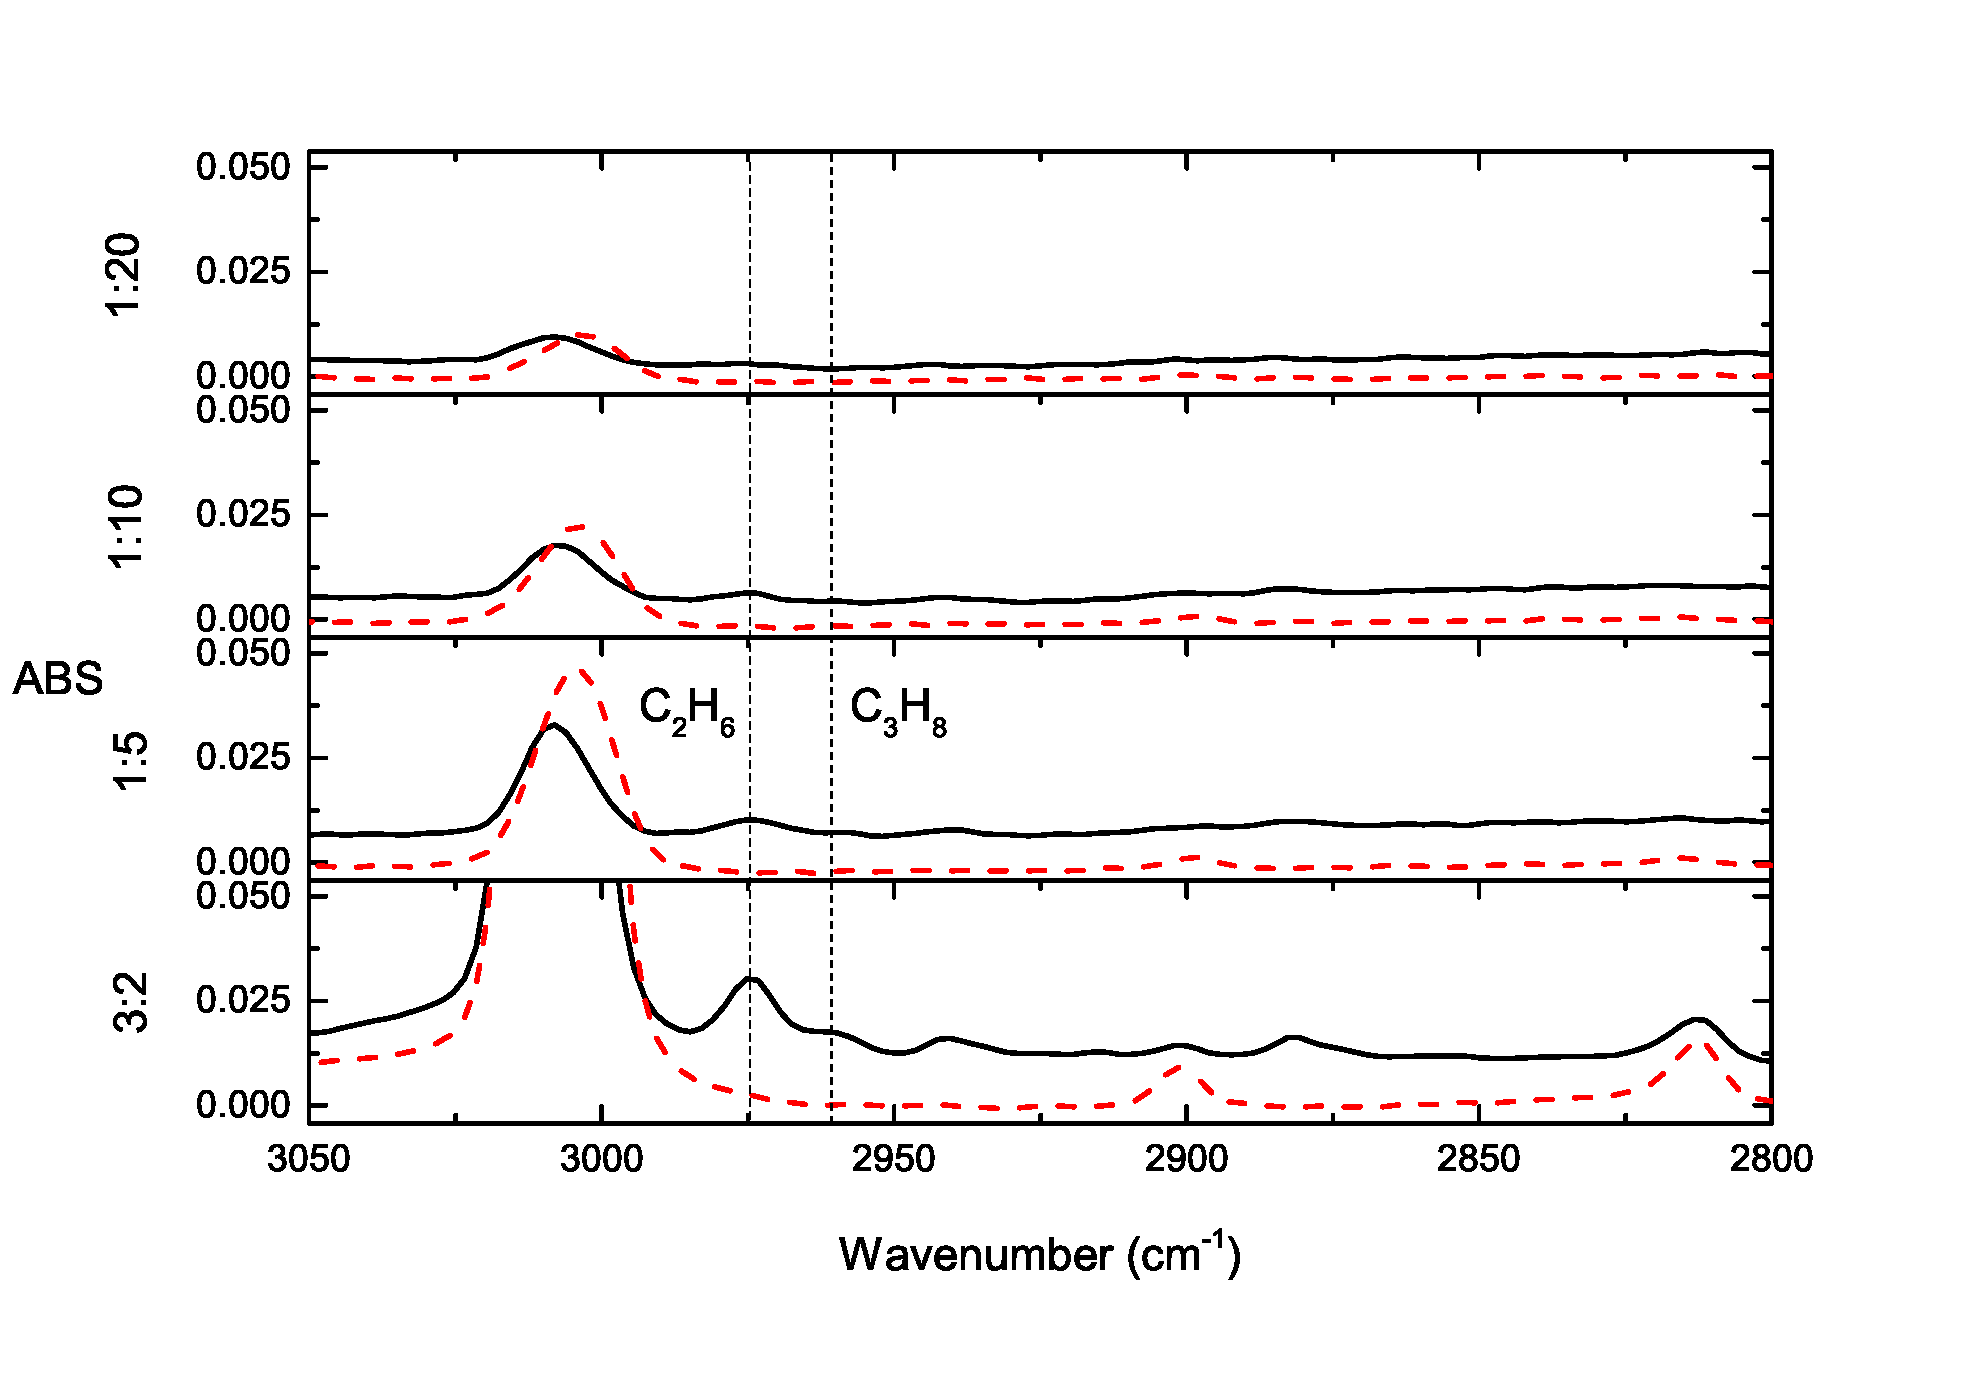
\includegraphics[width=\textwidth]{figures/chapter3/C2H6.eps}
\caption{The the infra-red spectrum of CH$_4$ + NH$_3$ ice mixtures of C$_2$H$_6$ and C$_3$H$_8$ before irradiation (dashed) and VUV irradiated ice mixtures provided by MDHL. }
\label{fig:C2H6}
\end{figure}

The assignment of C$_2$H$_6$ is confirmed by several bands listed in table \ref{tab:WavenumberMDHL}. Figure \ref{fig:C2H6} is a partial of figure \ref{fig:widerange}. The absorption peak located at 2075 cm$^{-1}$ is the strongest vibration of C$_2$H$_6$. The formation mechanism of C$_2$H$_6$ in astrophysical environment is proposed by Bennet et al. \cite{bennett2006laboratory}, that the main route to form C$_2$H$_6$ is by a combination of 2 CH$_3$ radicals (equation \ref{eq:CH3} and \ref{eq:C2H6}):

\begin{equation}
CH_4 + hv \rightarrow CH_3
\label{eq:CH3}
\end{equation}
\begin{equation}
2 CH_3 \rightarrow C_2H_6
\label{eq:C2H6}
\end{equation}

The energy required to produce 1 CH$_3$ radical from CH$_4$ is 4.42 eV. 2 CH$_3$ radicals recombine to form C$_2$H$_6$ releases 3.74 eV. Therefore, equation \ref{eq:C2H6} is a no-barrier exothermic process. However, C$_2$H$_6$ is not detected in CH$_4$+NH$_3$=1:20 ice mixtures. Figure \ref{fig:lab_C2H6} shows the temporal formation column density of C$_2$H$_6$ in different configurations of irradiated ice mixtures.  As the formation only depends on CH$_4$, we may use first order kinetics equation to fit the column density versus photon dose.
\begin{equation}
[A] = [A]_0(1 - e^{-k_1 t})
\label{eq:1step}
\end{equation}
to fit the formation of C$_2$H$_6$. The fitting results are shown in table \ref{tab:fittingC2H6}.

\begin{figure}
\centering
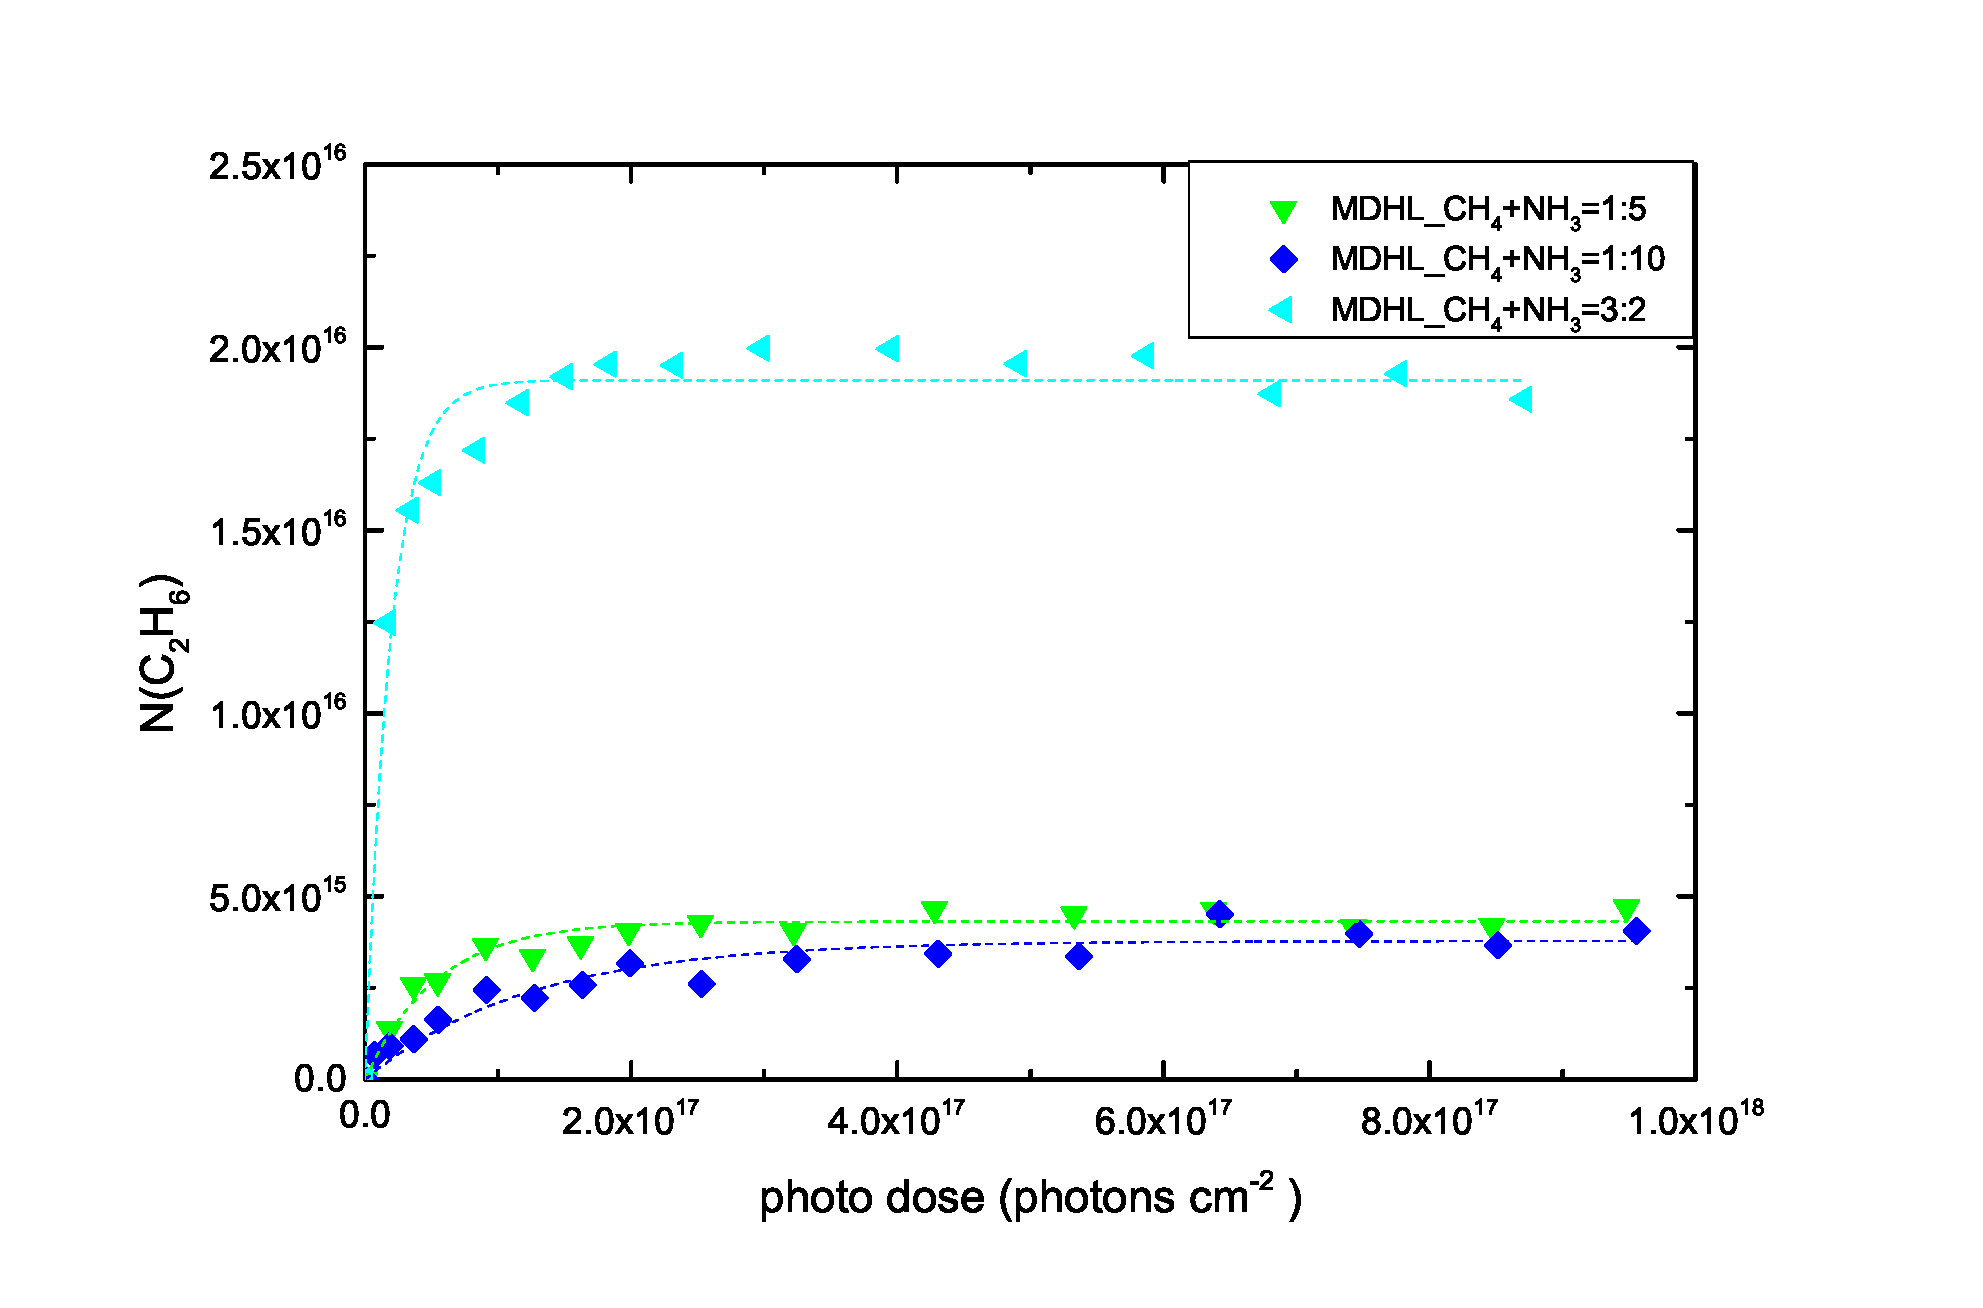
\includegraphics[width=\textwidth]{figures/chapter3/Lab_C2H6.eps}
\caption{The column density of C2H6 during CH4 + NH3 ice mixtures irradiated by MDHL. }
\label{fig:lab_C2H6}
\end{figure}

\begin{table}[htbp]
\caption{The fitting results of C$_2$H$_6$ by [C$_2$H$_6$]=[C$_2$H$_6$]$(1 - e^{-k_1 t})$}
\label{tab:fittingC2H6}
\begin{tabular}{ccc}
\hline
\hline
Ratio of CH$_4$+NH$_3$ & A (x10$^{15}$ molecules cm$^{-2}$) & k (x10$^{-17}$ photon$^{-1}$) \\
\hline
1:10 & 2.90 $\pm$ 1.25 & 0.92 $\pm$ 0.15 \\
1:5 & 4.16 $\pm$ 0.28 & 2.28 $\pm$ 0.28 \\
3:2 & 19.2 $\pm$ 0.15 & 5.28 $\pm$ 0.25 \\
\hline
\end{tabular}
\end{table}

From table \ref{tab:fittingC2H6}, production rate is also proportional to the initial CH$_4$ concentration.


\subsection{C$_3$H$_8$}

The peak positioned at 2960 cm$^{-1}$ belongs to –CH$_2$- so we assigned that as C$_3$H$_8$, as the shortest carbon chain. The signal to noise ratio in CH$_4$+NH$_3$ = 1:10 is poor that we can not quantize the amount of C$_3$H$_8$ (figure \ref{fig:C2H6}).

It is a secondary product formed by a combination of either C$_2$H$_6$ + CH$_2$ (equation \ref{eq:C3H81})or C$_2$H$_4$ + CH$_4$ (equation \ref{eq:C3H82}).
\begin{equation}
C_2H_6 + CH_2 \rightarrow C_3H_8
\label{eq:C3H81}
\end{equation}
\begin{equation}
C_2H_4 + CH_4 \rightarrow C_3H_8
\label{eq:C3H82}
\end{equation}

By modern peak fitting method, we deconvoluted the overlapped C$_2$H$_6$ and C$_3$H$_8$ into two gaussians.

\subsection{CN$^-$}

\begin{figure}
\centering
\includegraphics[width=\textwidth]{figures/chapter3/CN.eps}
\caption{The the infra-red spectrum of CH$_4$ + NH$_3$ ice mixtures of C$_2$H$_6$ and C$_3$H$_8$ before irradiation (dashed) and VUV irradiated ice mixtures provided by MDHL. }
\label{fig:CN}
\end{figure}

From infra-red absorption spectrum (figure \ref{fig:CN}) and their positions, we assigned the peak 2086 cm$^{-1}$ to CN$^-$  but not a combination of HCN and CN$^-$. The assignment is based on a absence in CN bending mode at 848 cm$^{-1}$. In the case CH$_4$ + NH$_3$ = 3:2, we may observe a peak located at 820 cm$^{-1}$, which is with a FWHM half of HCN and it is eliminated at 50 K during the warm-up phase. Since 50 K is the desorbing temperature of C$_2$H$_6$ and the peak position is the close to v12 mode of C$_2$H$_6$, we believe that the 820 cm$^{-1}$ peak is contributed by C$_2$H$_6$. Therefore, we may assign our peak located at 2086 cm$^{-1}$ as purely CN$^-$.\\

\begin{figure}
\centering
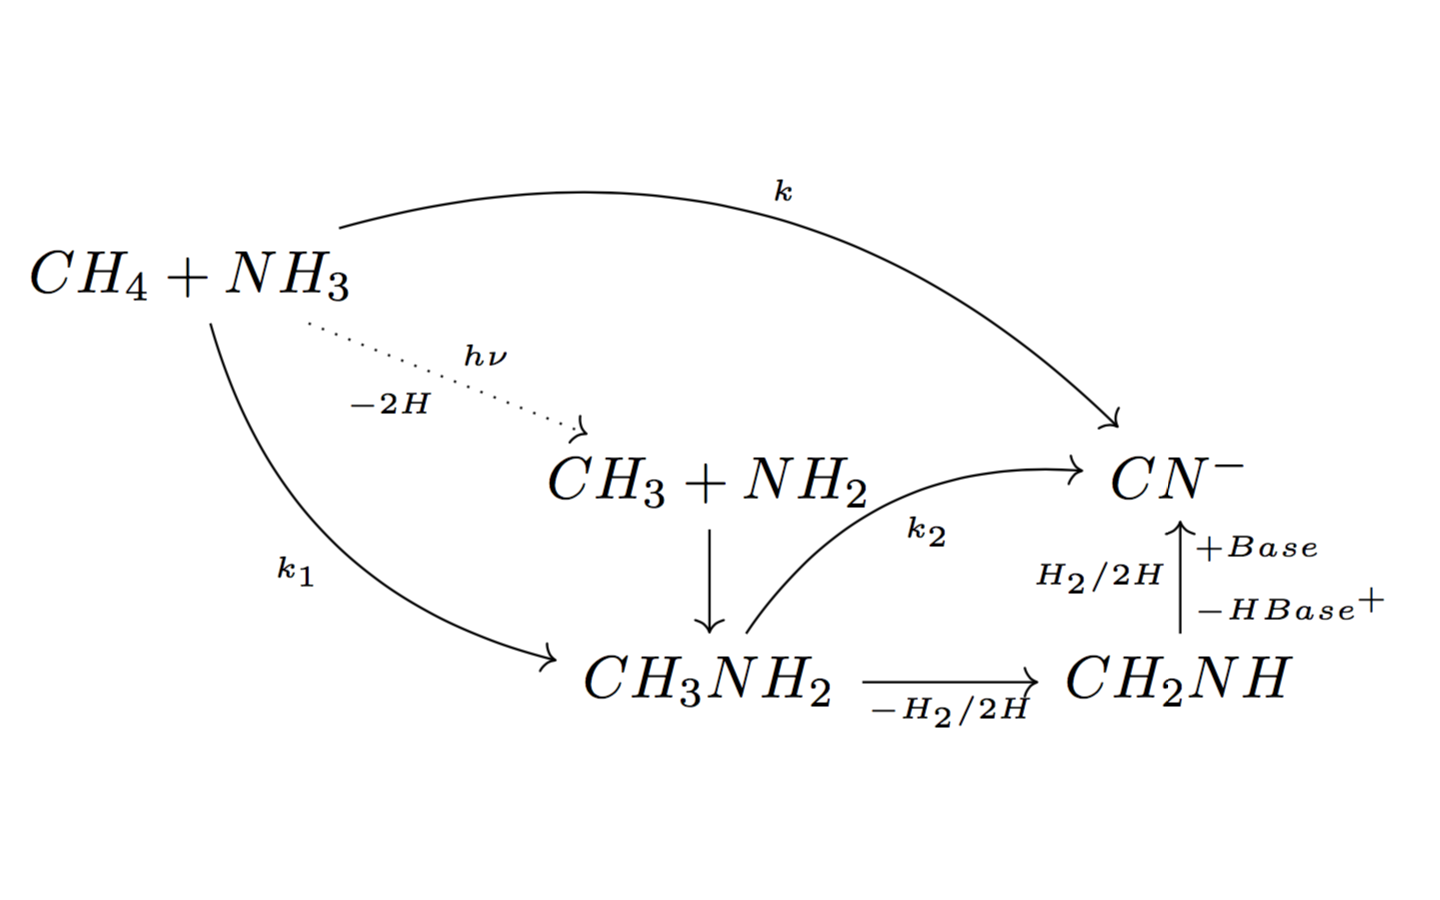
\includegraphics[width=\textwidth]{figures/chapter3/CNmechanism}
\caption{The formation mechanism of CN$^-$ proposed by Kim and Kaiser(2011). }
\label{fig:CNmechanism}
\end{figure}

The formation mechanism of CN$^-$ at low temperature was first suggested by Kim and Kaiser (2011) to be two step reaction mechanism with methylamine as intermediate. CH$_4$ and NH$_3$ irradiated by photon to become CH$_3$ and NH$_2$ radical (figure \ref{CNmechanism}, followed by propagation and recombination of radicals becoming CH$_3$NH$_2$ and dehydrogenation and acid-base reaction to form CN$^-$.
Although Kim and Kaiser used 1.5keV electron as energy source to simulate the cosmic ray induced photochemistry, this formation mechanism also applies in our photon irradiation experiments because we can also detect the methylamine during our warm-up phase. The ion fragment with m/z=31 is assigned as CH$_3$NH$_2$$^+$ and detectable in all ratios of our CH$_4$+NH$_3$ experiments (figure \ref{Mass31}).

\begin{figure}
\centering
\includegraphics[width=\textwidth]{figures/chapter3/Mass31.eps}
\caption{The m/z=31 detected by QMS during warm-up with heating rate 1 K/min in different configurations of ice mixtures.}
\label{fig:CNmechanism}
\end{figure}

By the deviation performed in section \ref{sec:Reaction_Rate_Laws}, we have a rate equation for consecutive reactions \ref{eq:rate7}. With one of the reactant larger than another, we applied the pseudo first order assumption. With equation \ref{eq:rate7}, we fitted the formation of CN$^-$ (figure \ref{fig:CNrate})and found that one of the rate constant is always larger than the other in all of the ratios. The fitting results are averaged by more than two experiments and are shown in table \ref{tab:CNrate}.The results of Kim and Kaiser is also listed into the table, they could observe a two-step reaction mechanism in production of CN$^-$ in CH4+NH3 (3:1) experiments with electron current 0.1 μA. However, when they increased the electron flux to 1 μA for irradiation C$_n$H$_{2n+2 (n=1-6)}$ and NH$_3$ ice mixtures, they also observed a one-step reaction mechanism.

\begin{figure}
\centering
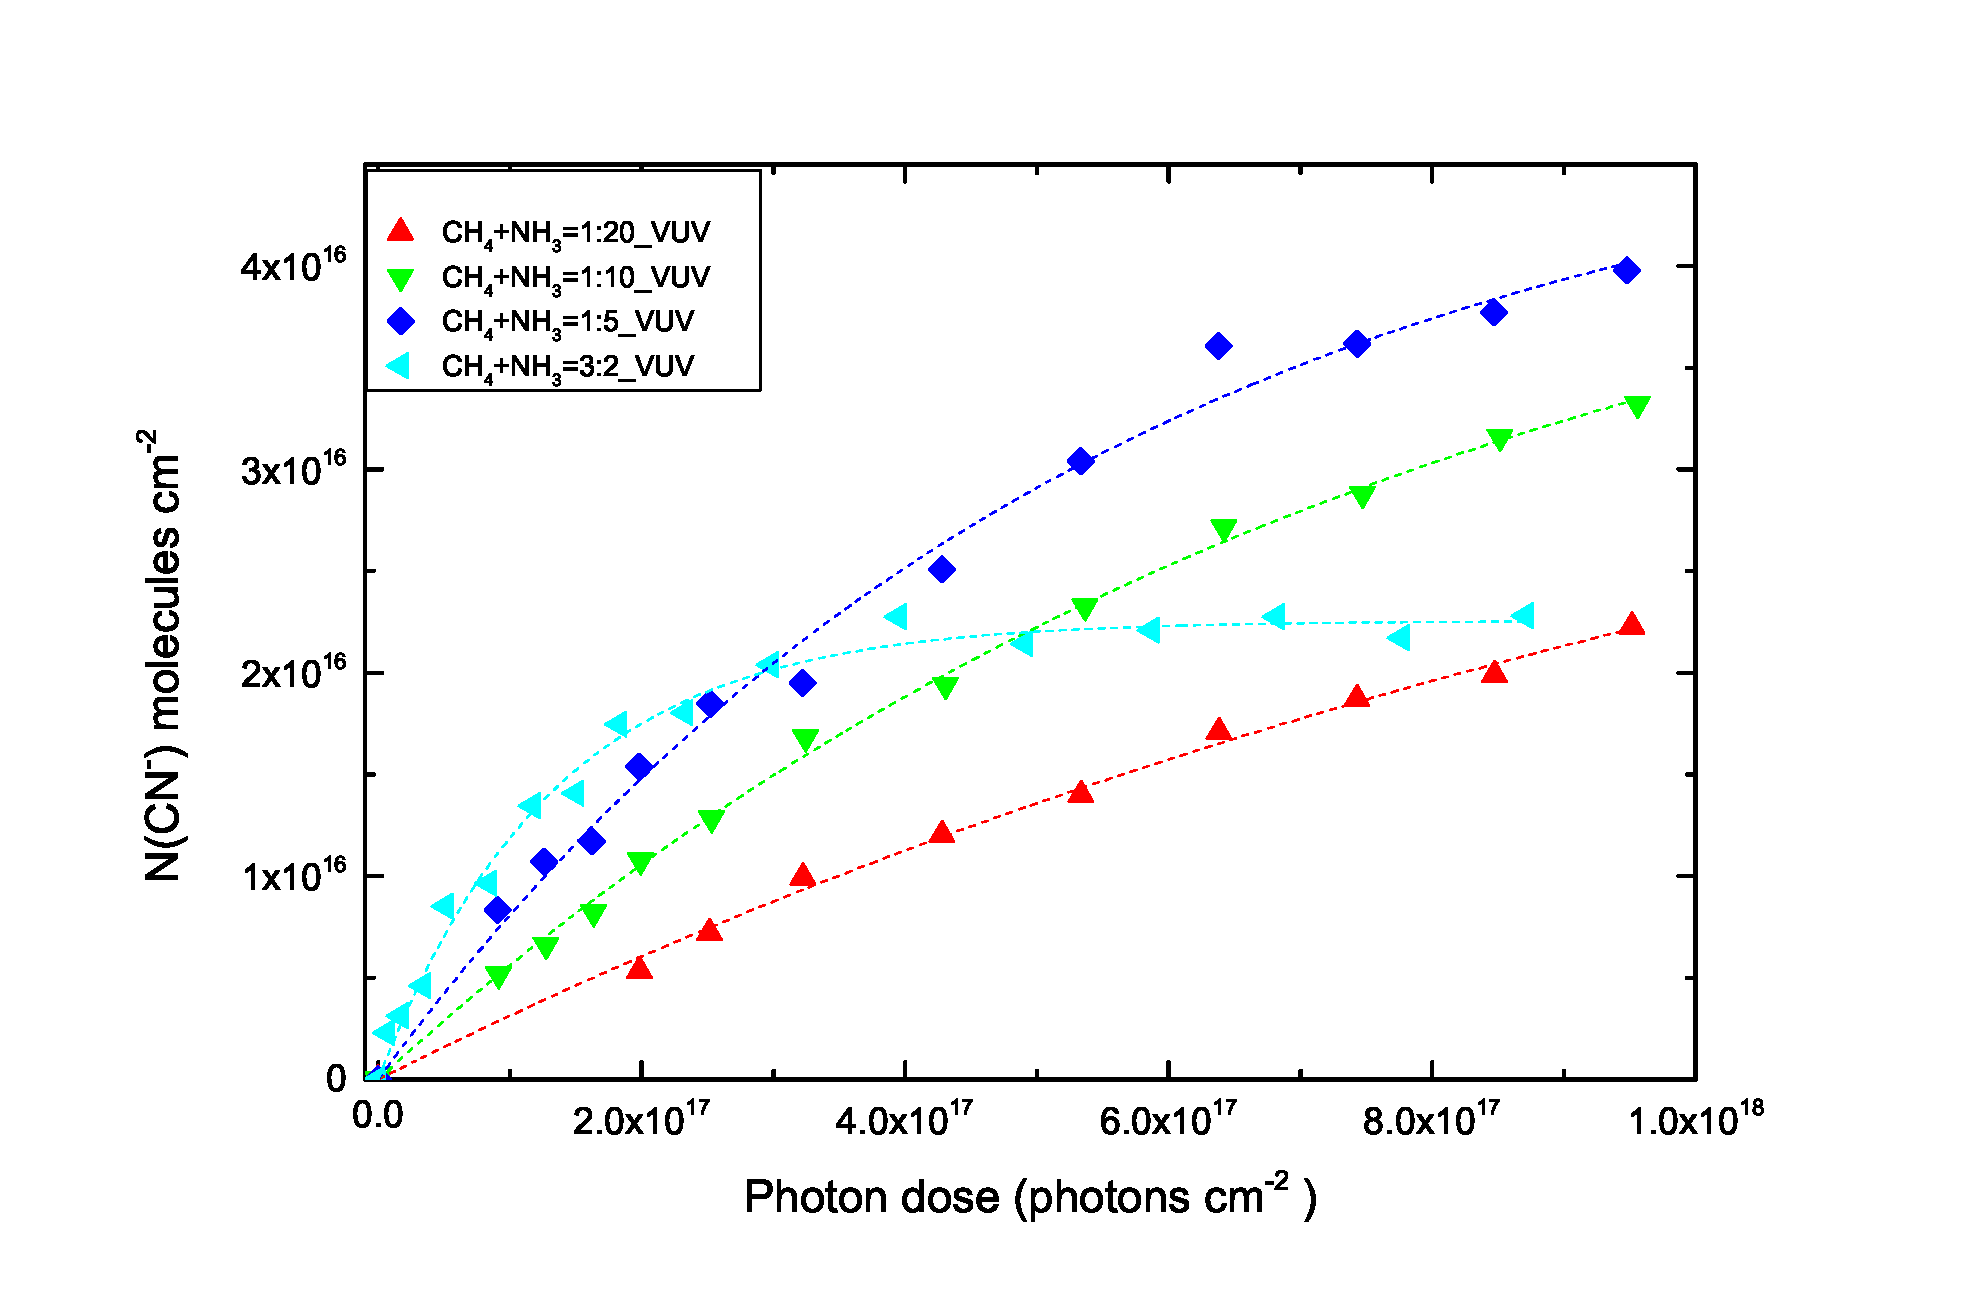
\includegraphics[width=\textwidth]{figures/chapter3/Overall_CN_rate.eps}
\caption{The column density of CN$^-$ accumulated when different configurations of CH$_4$ + NH$_3$ ice mixtures are irradiated by VUV photons provided by MDHL. The dotted lines are fits of column densities by equation \ref{eq:rate7}.}
\label{fig:CNrate}
\end{figure}

\begin{table}[htbp]
\caption{The fitting results of CN$^-$ by equation \ref{eq:rate7}}
\label{tab:CNrate}
\begin{tabular}{cccc}
\hline
\hline
Ratio of CH$_4$+NH$_3$ & A (x10$^{16}$ molecules cm$^{-2}$) & k$_1$ (x10$^{-18}$ photon$^{-1}$) & k$_2$ (photon$^{-1}$)\\
\hline
1:20 & 4.75 $\pm$ 0.40 & 0.70 $\pm$ 0.09 & >1 \\
1:10 & 4.51 $\pm$ 0.18 & 1.33 $\pm$ 0.13 & >1 \\
1:5 & 4.61 $\pm$ 0.18 & 1.93 $\pm$ 0.19 & >1 \\
3:2 & 2.24 $\pm$ 0.03 & 8.21 $\pm$ 0.70 & >1 \\
\hline
\end{tabular}
A represents the amount of CN$^-$ we may obtain when irradiated the ice for infinitely long.\
\end{table}

\section{The Concentration Effect in formation of Cyanide ions and Ethane}

\subsection{Cyanide ion}

From table \ref{tab:CNrate}, we may see that the rate k$_1$ is proportional to the concentration of CH$_4$. The rate constant k$_1$ increases when concentration of CH$_4$ increases. Since NH$_3$ is fixed in all of our experiments, more CH$_4$ are evolved into CH$_3$ radical formation when proportion of CH$_4$ in the ice mixture increases. More abundant CH$_3$ radicals in the ice mixtures would produce more CH$_3$NH$_2$ intermediates.

In CH$_4$+NH$_3$ =3:2 ice mixtures, A is half of the other ratios. The reduction is mainly because CN$^-$ has a competing relationship with formation of C$_2$H$_6$ and C$_3$H$_8$. NH$_2$ radicals competes with CH$_2$, CH$_3$ and C$_2$H$_4$ radicals. With this competition, the intermediate CH$_3$NH$_2$ is reduced. Therefore, in ratio 3:2 CH$_4$+NH$_3$ ice mixture, the yield of CN$^-$ is the least(table \ref{tab:CNrate}). Note that the formation yield of C2H6 is the maximum in this ratio (table \ref{tab:fittingC2H6})


Considering the normalized CN$^-$ with respect to the initial CH$_4$(figure \ref{fig:CN_CH4}), the formation of CN$^-$ is more effective in low CH$_4$ concentration ice mixtures. The mobile CH$_3$ radical is aggregated by excess NH$_3$. In this situation, CH$_3$ radicals have less chance to meet another CH$_3$ radical or C$_2$H$_4$. It is more likely to react with NH$_2$ radicals so the formation of CN$^-$ in low CH$_4$ concentration ice mixtures are more efficient.

\begin{figure}
\centering
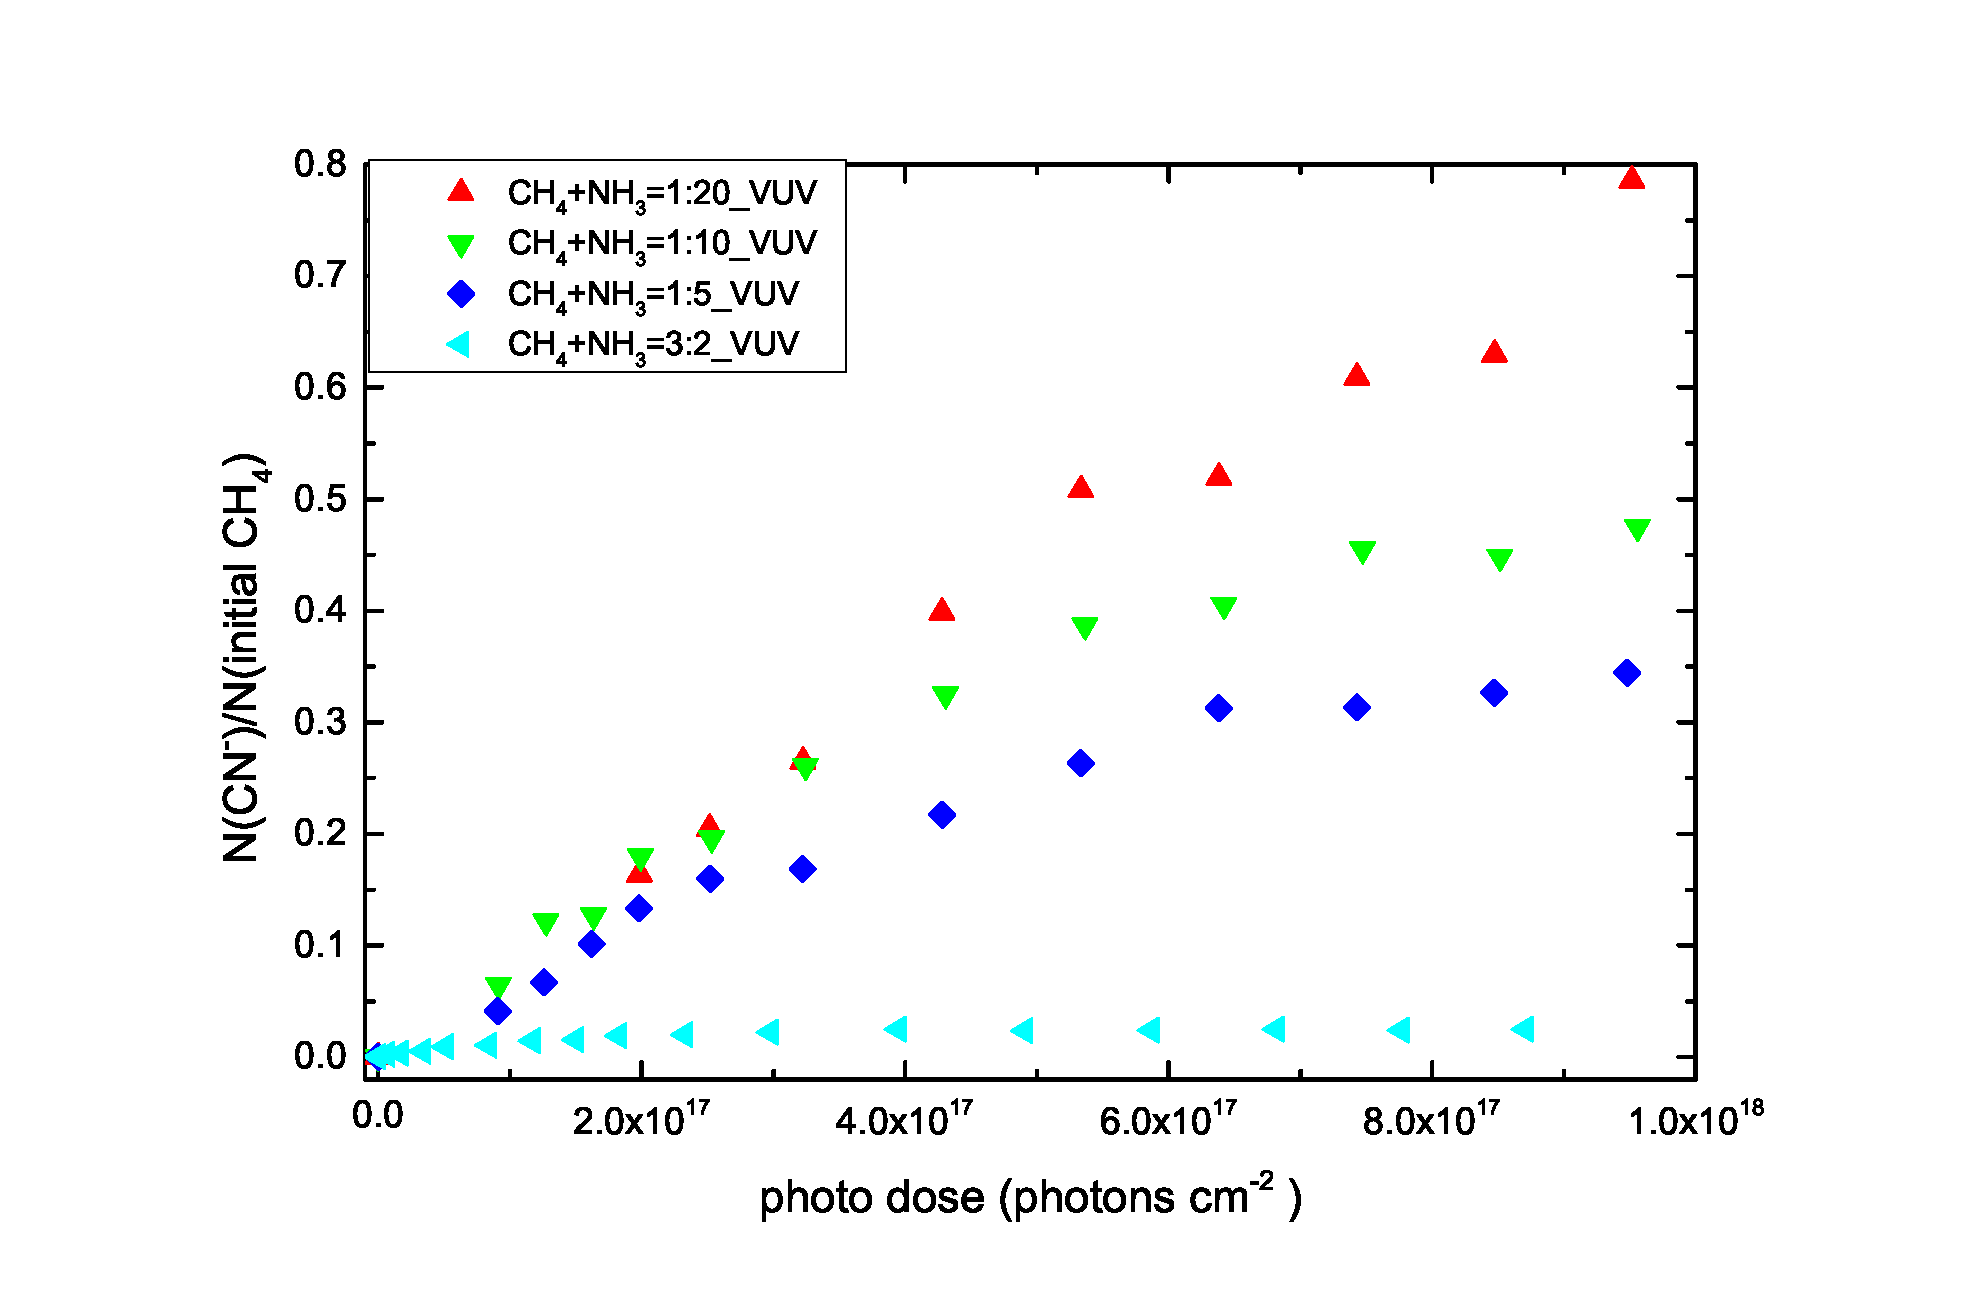
\includegraphics[width=\textwidth]{figures/chapter3/CN_CH4.eps}
\caption{The column density of CN$^-$ divided by initial CH$_4$ accumulated when different configurations of CH$_4$ + NH$_3$ ice mixtures are irradiated by VUV photons provided by MDHL.}
\label{fig:CN_CH4}
\end{figure}

\subsection{Ethane}


\begin{figure}
\centering
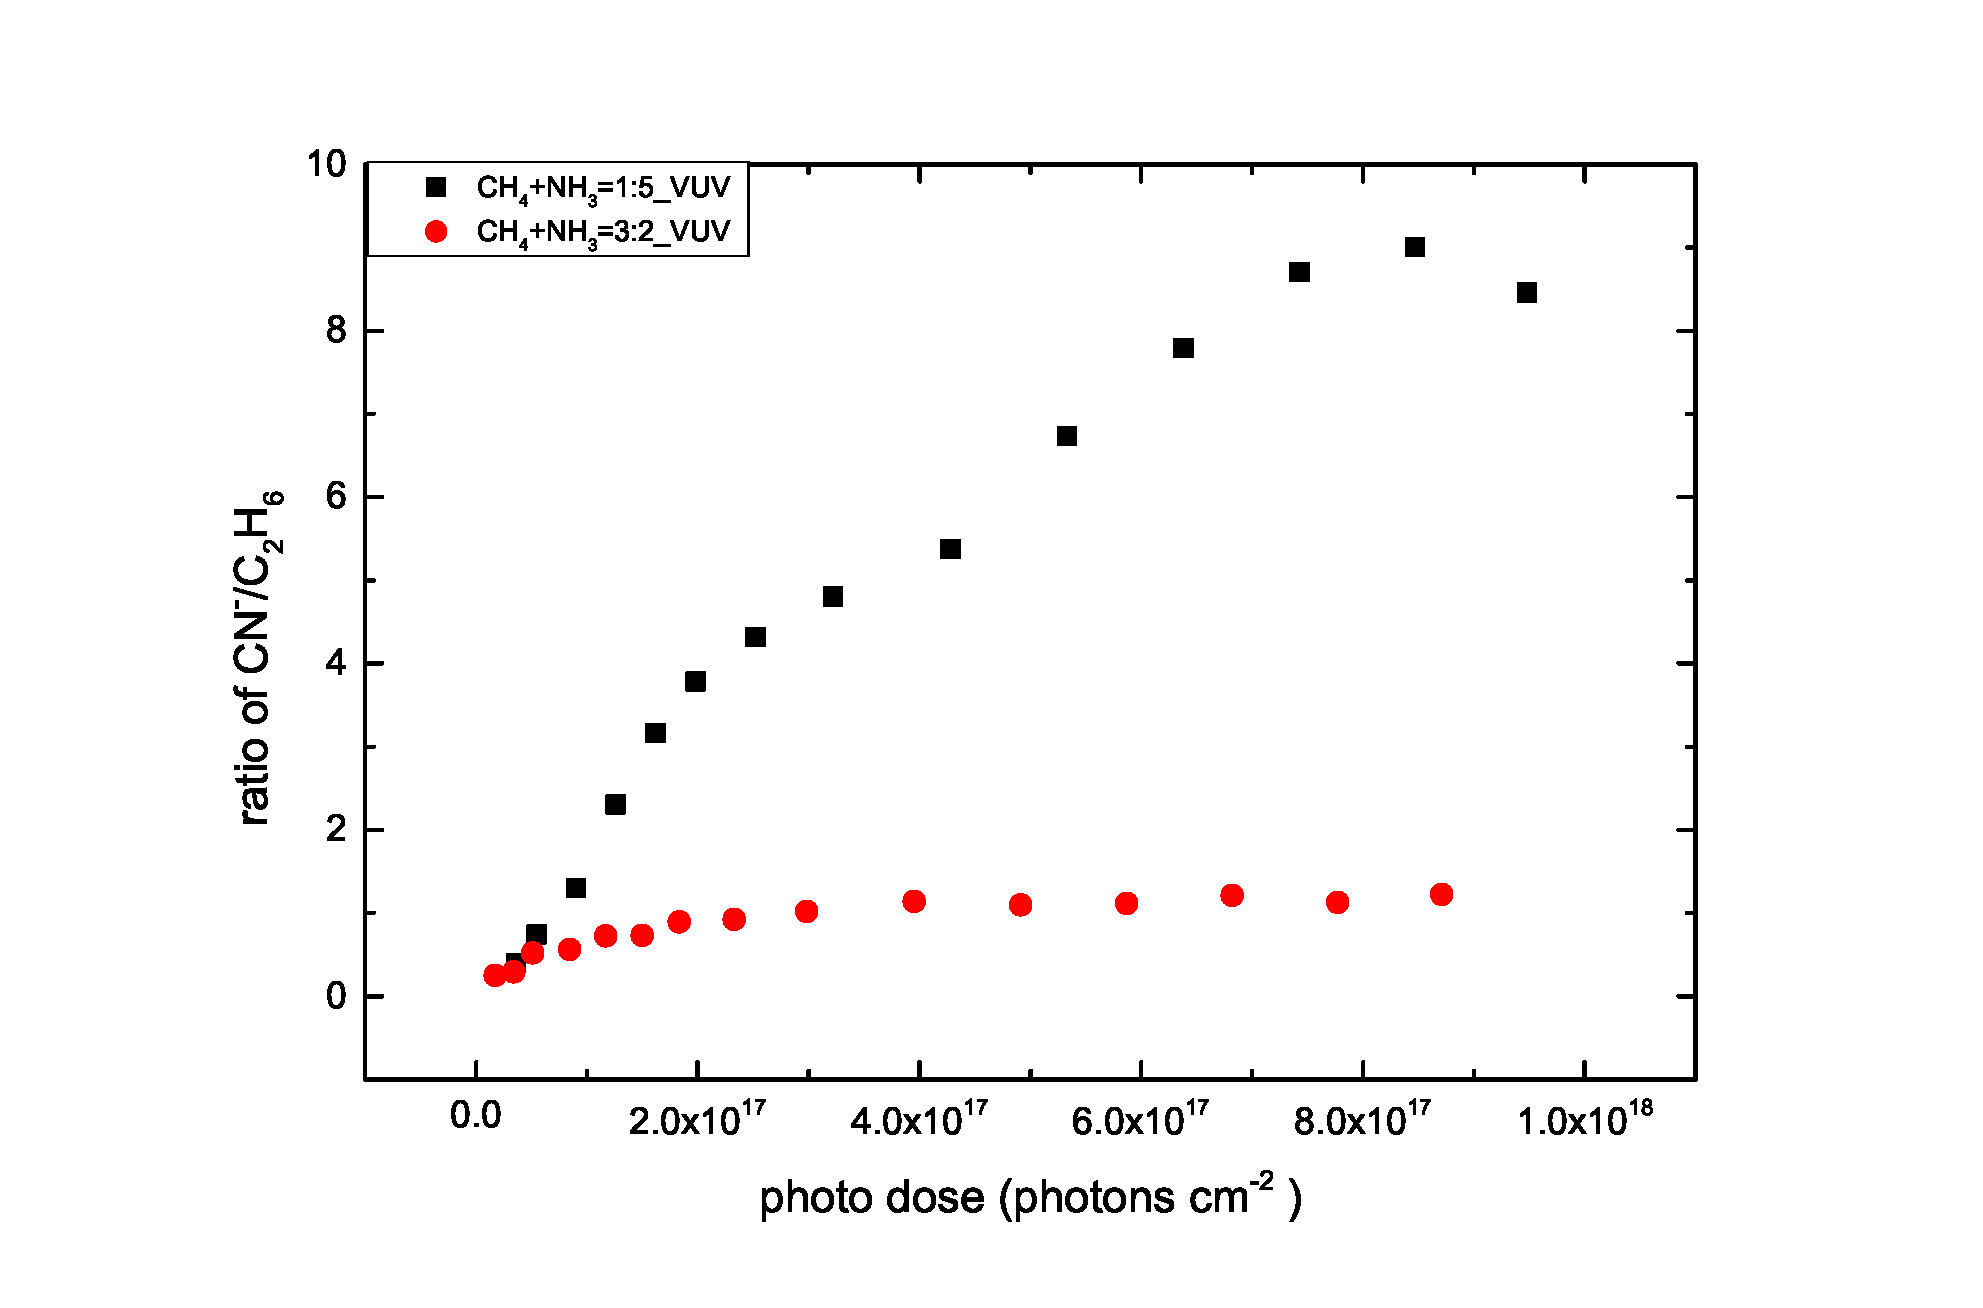
\includegraphics[width=\textwidth]{figures/chapter3/CN_C2H6.eps}
\caption{The column density of CN$^-$ divided by C$_2$H$_6$ accumulated when different configurations of CH$_4$ + NH$_3$ ice mixtures are irradiated by VUV photons provided by MDHL.}
\label{fig:C2H6_CN}
\end{figure}

Considering the case of ratio of CN$^-$ divided by C$_2$H$_6$,the formation of CN$^-$ in ice mixtures with diluted CH$_4$ has more CN$^-$ formed then C$_2$H$_6$. It is because ice mixtures with with higher concentrations in CH$_4$ is more effective for one CH$_3$ radical to combine with another CH$_3$ radical. On the contrast, CH$_3$ radicals formed in the ice mixtures with diluted CH$_4$ concentrations are aggregated by NH$_3$. Therefore, CN$^-$ is less efficient to form in ice mixtures with excess NH$_3$.

\subsection{Propane}

\begin{figure}
\centering
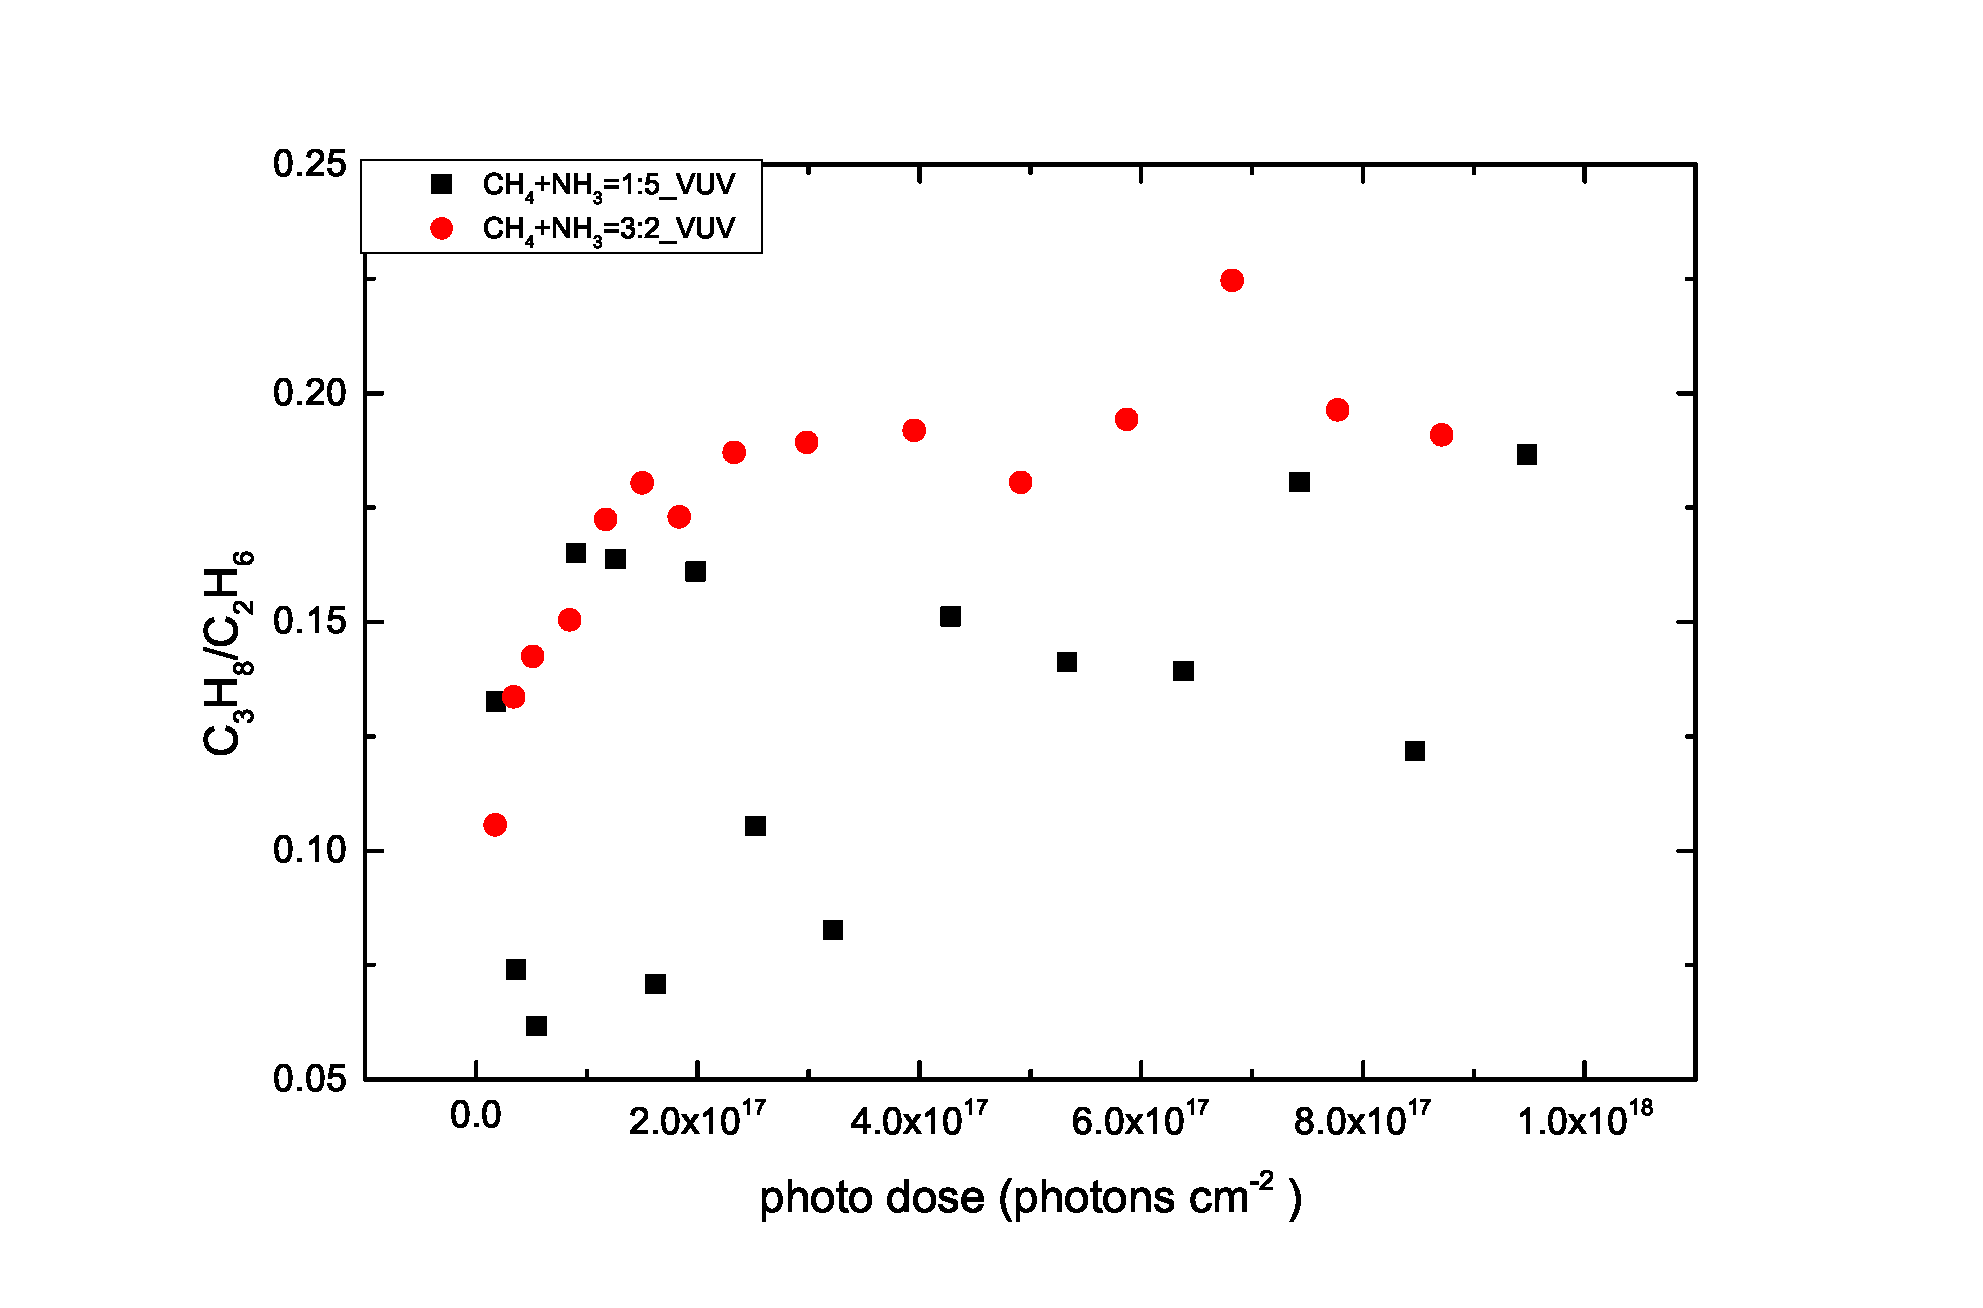
\includegraphics[width=\textwidth]{figures/chapter3/Lab_C3H8_C2H6.eps}
\caption{The column density of C$_3$H$_8$ divided by C$_2$H$_6$ accumulated when different configurations of CH$_4$ + NH$_3$ ice mixtures are irradiated by VUV photons provided by MDHL.}
\label{fig:C2H6_C3H8}
\end{figure}

C$_3$H$_8$ forms based on to the C$_2$H$_6$ \ref{fig:C2H6_C3H8} is the plot with column densities of C$_2$H$_6$ divided by C$_3$H$_8$. We may see that the ratio in CH$_4$+NH$_3$ =1:5 experiment is around 6 where CH$_4$+NH$_3$ =3:2 is around 3. This shows that the amount of C$_3$H$_8$ in CH$_4$+NH$_3$ =3:2 experiment is higher. It is rather difficult for C$_3$H$_8$ to form in CH$_4$+NH$_3$ = 1:5 experiments because NH$_3$ aggregated them. The formation of C$_3$H$_8$ in CH4+NH3 =1:5 and 3:2 experiments has given a reasonable explanation about why C$_2$H$_6$ formation is most efficient in CH$_4$+NH$_3$ =1:10 experiments.

\section{Cyanide ion produced by photon source and electron source}

We study the ice mixtures of CH$_3$ dominated ice mixtures and compare the efficencies in CN%^-% formation by electrons and VUV irradiations.  Ice thickness and energy conversion is important to study the yield of the products. First, we compare the ice thicknesses. The only ice mixture with CH$_4$ dominating  and experiments done by Kim and Kaiser (2011).

We calculated the percentage of photons absorbed by CH$_4$+NH$_3$ ice mixtures in different configurations. Applying cross-sections measured by Cruz-Diaz et al. (2014) and the spectrum of our MDHL and substitute them into Beer’s law. In CH$_4$+NH$_3$ = 3:2 ice mixtures with ammonia fixed at 600 ML can absorb more than 99.9 \% of light. Therefore, we may assume all the irradiated light is absorbed by the ice. For CH$_4$+NH$_3$ =3:2 ice mixture, around 9 $\times$ 10$^{17}$ photons were irradiated in 270 minutes.

In Kim and Kaiser (2011) electron irradiation experiments, the energy transferred to CH$_4$ + NH$_3$ ice mixtures is by linear electron transfer (LET) that 1.3 eV molecule$^{-1}$ was absorbed by the ice in 90 minutes. They get flattened at 20 minutes’ irradiation, with fluence of 2.0 $\times$ 10$^{14}$ electrons cm$^{-2}$. While we got flattened at a dose of 3 $\times$ 10$^{17}$ photons cm$^{-2}$. Considering the energy of their electron (1.5 keV) and energy of our photons, they got flattened at 3 $\times$ 10$^{17}$ eV cm$^{-2}$ while we get flattened at 27.81 $\times$ 10$^{17}$ eV cm$^{-2}$. Comparing these energy doses, less electrons are needed to flatten the formation of CN$^-$.

Comparing our CN$^-$ obtained after infinitely long exposure, 13 – 16 ML of CN$^-$ was obtained by electron irradiation depending on which equation they choose to fit. In our MDHL experiments, we have 14.8 ML of CN$^-$. However, Kim and Kaiser (2011) adopted the CN$^-$ absorption coefficient measured by Georgieva and Velcheva (2006) to be 3.7 x 10$^{-18}$ cm molecule$^{-1}$, which is 4.86 times smaller. We do not adopt this absorption coefficient because it violates the carbon balance that number of CN$^-$ produced will be larger than CH$_4$ consumption. If we adopted the same absorption coefficient, the production yield of CN$^-$ should be multiplied by 4.86. Therefore, our yield is 72 ML of CN$^-$. Regarding percentage of NH$_3$ (limiting reactant), Kim and Kaiser has 5 - 6 \% yield where we have 12 \% yield if we adopted the same absorption coefficients. To conclude, electron irradiation has a smaller absorption cross-sections, the percentage of yield is also smaller than VUV irradiated ice mixtures with similar ice thicknesses.




\section{Photon Energy Effect - EUV and VUV}

According to Blanksby and Ellison, the dissociation energy for CH$_4$, becoming CH$_3$, CH$_2$ CH and C are 4.55, 4.79, 4.39 and 3.51 eV respectively at 298 K. Whereas dissociation energy for NH$_3$, becoming NH$_2$ is 4.67 eV at 298 K.

Considering our MDHL with average energy of 9.27 eV, all of the above fragments may exist rather in the form of radicals or combined with other radicals to form heavier molecules in our ice mixtures. It is not nessesary to further increase the photon energy in order to get another new fragmentation pathway. However, the fragmentation of CH$_4$ and NH$_3$ depends on photon energy.

Several gaseous state measurements also presents this result. First, gans et al. (2011) changed photon wavelengthes from 121.6 nm to 118.2 nm to dissociate the CH$_4$ molecules and ionize the fragments with the corresponding photon energy. Changing from 121.6 to 118.1 nm significantly changed the ionized fragmentation ratio from CH$_3^+$ and CH$_2^+$ ~ 1: 1 to 1:2 using pulsed laser. This slightly change of photon energy, from 10.2 eV to 10.4 eV has a significant change in the fragmentation of CH4.

Second, Tsai et al. used 30.4 nm to photo dissociate CH$_4$ and test it by time – of – flight mass spectrometer yields CH$_3^+$: CH$_2^+$: CH$^+$: C$^+$ = 1 :0.32: 0.118: 0.0237 (Tsai 1980). Since it is also a gaseous state experimental results, we cannot directly apply this fragmentation into our calculations. Note that the VUV absorption spectra of CH$_4$ in solid phases is different from gaseous phases (Cruz-Diaz 2014), so the exact photo dissociation fragmentation ratios by 30.4 nm nor VUV irradiations in astronomical environments are still unknown.

Thirdly, a group also varies ratios of CH$_4$ + NH$_3$ mixtures and irradiate with far UV irradiation at 134 nm (Bossard 1980). However, this group only used gas chromatography to analyse the final products and their reaction is carried in gas phase in room temperature. Although the photon energy of our MDHL is enough to dissociate both the CH$_4$ and NH$_3$ molecules, we further increase photon energy to He II 30.4 nm to examine whether there are differences in photo-products. It is worthwhile for us to perform experiment by EUV irradiation to see if the EUV irradiation can generate any new products on the surface of Charon, or any difference in yield. After investigation, we may answer several questions: Are there any differences in products or production yields? Would the formation mechanism change?

\begin{figure}
\centering
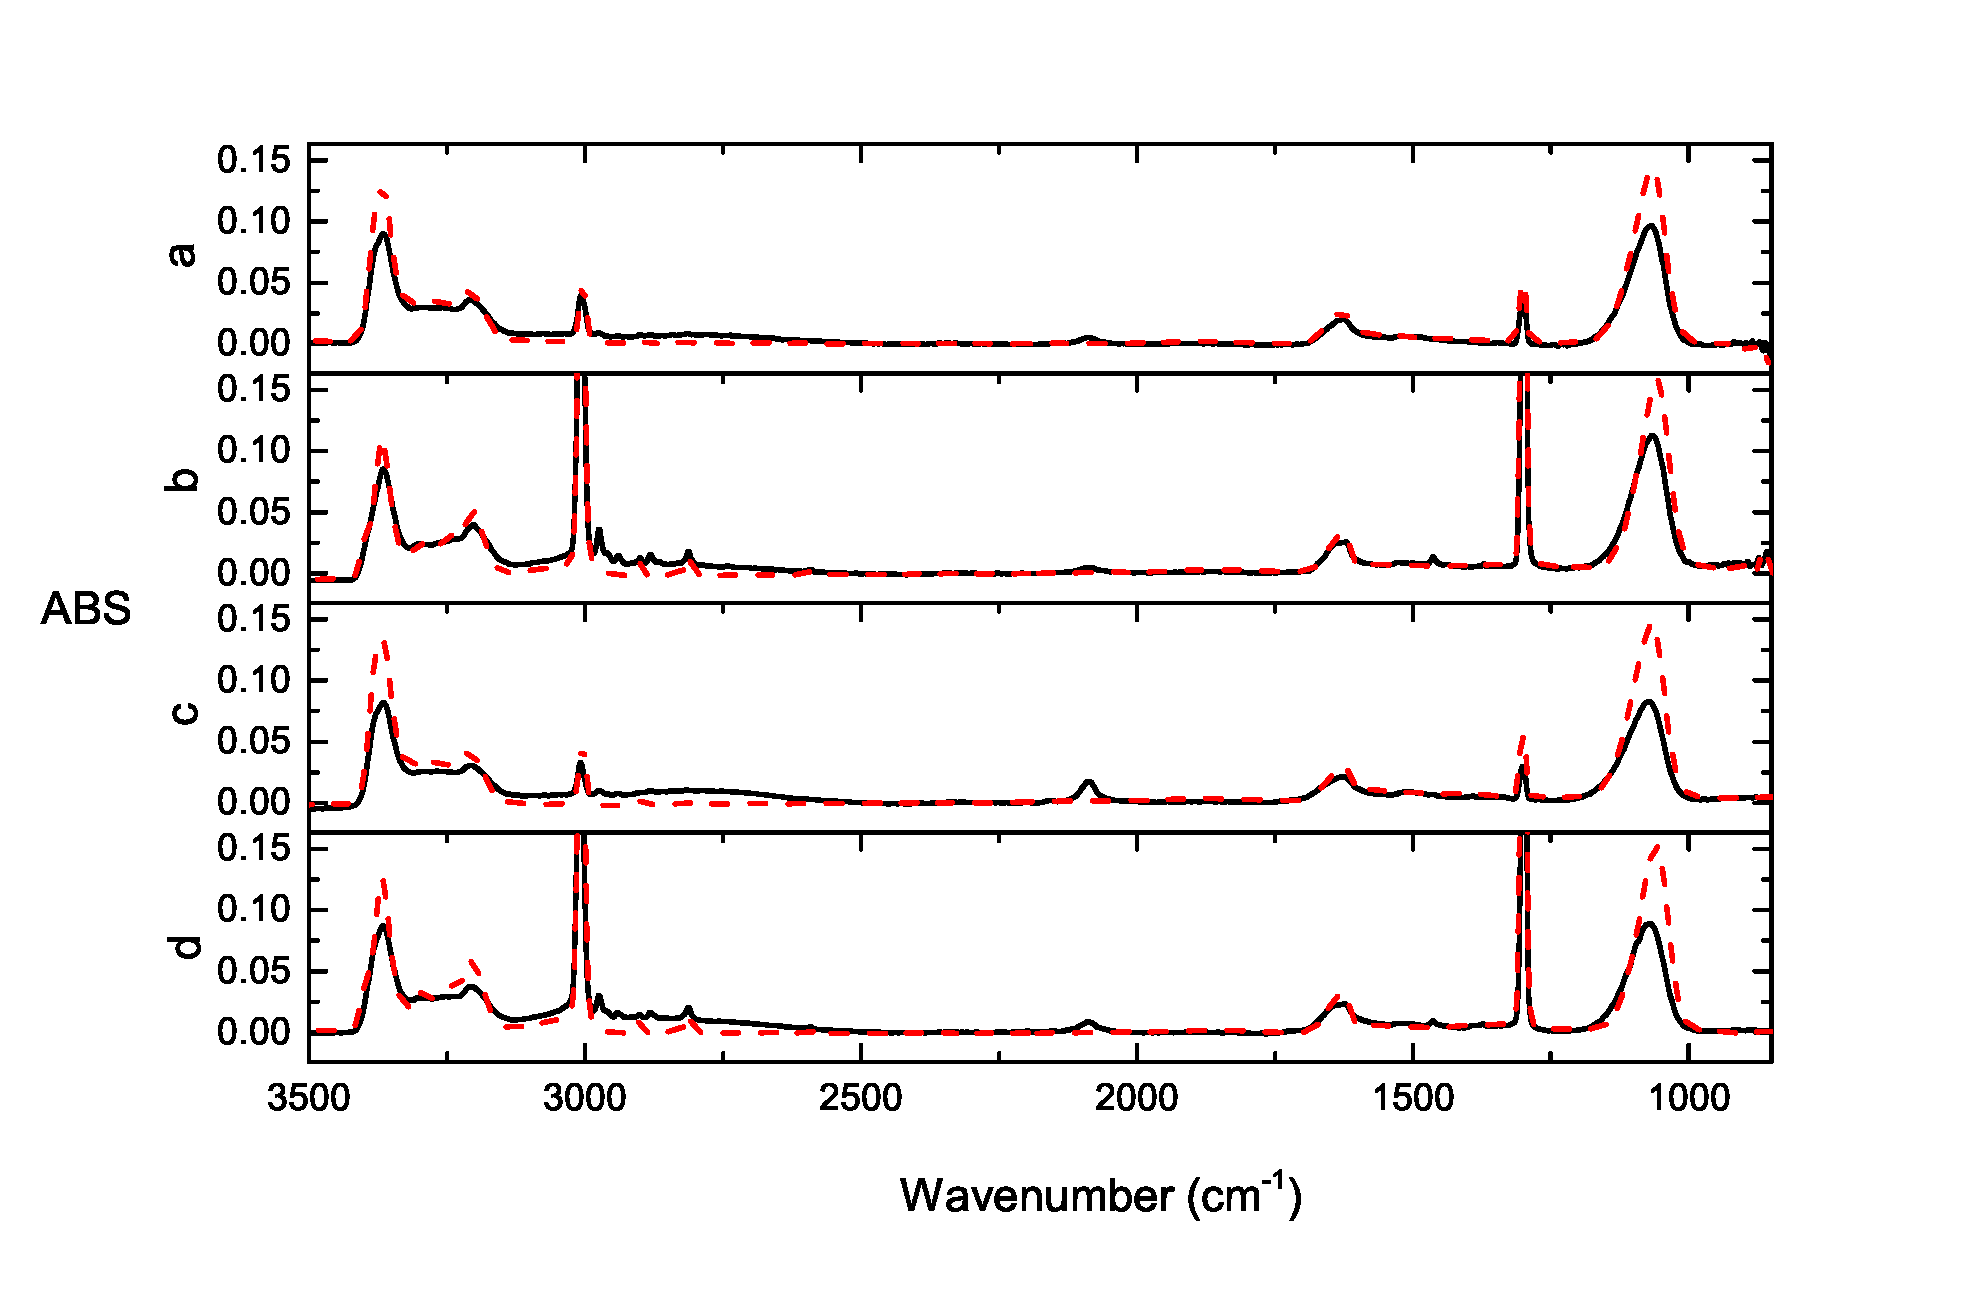
\includegraphics[width=\textwidth]{figures/chapter3/NSRRC_MDHL_IR.eps}
\caption{The the infra-red spectrum of CH$_4$ + NH$_3$ ice mixtures before irradiation (dashed) and VUV and EUV (solid) irradiated ice mixtures provided by MDHL. (a) and (b) are EUV irradiated CH$_4$+NH$_3$ = 1:5 and 3:2 ice mixtures respectively, and (c) and (d) are VUV irradiated CH$_4$+NH$_3$ = 1:5 and 3:2 ice mixtures respectively.}
\label{fig:NSRRC_MDHL_IR}
\end{figure}

Table \ref{tab:WavenumberNSRRC} shows the identified peaks of CH$_4$+NH$_3$ ice mixtures irradiated by VUV and EUV (30.4 nm) irradiated in IR spectra (figure \ref{fig:NSRRC_MDHL_IR}).

\begin{table}[htbp]
\caption{The peak positions of identified substances after VUV and EUV irradiations in different configurations of ice mixtures.}
\label{tab:WavenumberNSRRC}
\begin{tabular}{ccccccc}
\hline
\hline
\multicolumn{2}{c}{Literture assignments} & \multicolumn{2}{c}{CH$_4$+NH$_3$ ratio (MDHL)} & \multicolumn{2}{c}{CH$_4$+NH$_3$ ratio (30.4 nm)} \\
\hline
Wavenumber & Carrier  & 1:5 & 3:2 & 1:5 & 3:2 & Ref. \\
(cm$^{-1}$) &   & (cm$^{-1}$) & (cm$^{-1}$) & (cm$^{-1}$) & (cm$^{-1}$) &\\
\hline
3375 & $\nu_3$ (NH$_3$) & 3366 & 3367 & 3368 & 3368 & 1 \\
3290 & $2\nu_4$ (NH$_3$) & - & - & - & - & 1 \\
3210 & $\nu_1$ (NH$_3$) & 3207 & 3205 & 3209 & 3205 &1 \\
3011 & $\nu_3$ (CH$_4$) & - & - & - & - & 2 \\
2972 & $\nu_{10}$ (C$_2$H$_6$) & 2975 & 2975 2977 & 2976 & & 3 \\
2960 & C$_3$H$_8$ & - & 2960 & - & 2960 & 7 \\
2941 & $\nu_8+\nu_11$ (C$_2$H$_6$) & 2940 & 2940 & - & 2942 & 3 \\
2904 & $\nu_1$ (CH$_4$) & 2901 & 2901 & 2901 & 2901 & 5 \\
2879 & $\nu_5$ (C$_2$H$_6$) & 2882 & 2882 & - & 2884&  3 \\
2814 & $\nu_2+\nu_4$ (CH$_4$) & - & 2815 & - & 2813 & 5 \\
2083 & $\nu$ (CN$^-$) & 2088  & 2088 & 2090 & 2089 & 2 \\
1625 & $\nu_4$ (NH$_3$) & 1625 & 1631 & 1627 & 1631 & 1 \\
1514 & $\delta$ (NH$_2$) & 1509 & 1511 & 1509 & 1511 & 6 \\
1465-1440 & deform CH$_2$ scissor & 1461 & 1463 & - & 1465 & 3,4 \\
1390-1370 & CH$_3$ sym deform & 1394 & 1372 & - & 1372 & 4 \\
1298 & $\nu_4$ (CH$_4$) & 1301 & 1299 & 1303 & 1301 & 2 \\
1075 & $\nu_2$ (NH$_3$) & 1073 & 1072 & 1070 & 1068 & 1 \\
820 & $\nu_12$ (C$_2$H$_6$) & - & 820 & - & - & 3 \\
\hline
\end{tabular}\\
Reference: 1. Bossa et al 2008 2. Moore and Hudson 2003 3. Kim et al. 2010 4. Socrates 2001 5. Bennet and Kaiser 2007 6. Zheng et al. 2008 7. Hudson and Moore 2004
\end{table}


Considering the formation mechanisms of C$_2$H$_6$ and C$_3$H$_8$, equation (\ref{eq:C2H6} and \ref{eq:C3H81}), when changing the photon source from MDHL VUV irradiation to He II 30.4 nm monochromatic light to irradiate CH$_4$+NH$_3$ (3:2) ice mixtures, the ratio of C$_2$H$_6$ / C$_3$H$_8$ of ice mixtures irradiated by VUV irradiation is lower than EUV irradiation provided by NSRRC (figure 3.2.1). There are two probable explanations. First, the fragmentation of CH$_4$ is different with different photon energies. Therefore, less C$_3$H$_8$ is produced with EUV photons. Second, the destruction of CH4 is much less efficient by EUV irradiation. Therefore, the CH$_3$ radicals are not as rich as the ice mixture irradiated by VUV photons provided by the MDHL. As a result, we further irradiate our ice mixtures by EUV photons until the destruction of CH$_4$ is similar to VUV irradiation experiments done with MDHL. We found that the second explanation is more persuasive because after CH4 destruction equals to VUV irradiation, the ratio of C$_2$H$_6$/C$_3$H$_8$ of average of last 7 irradiations is 3.53 and 3.66 in experiments done with 3 experiments with MDHL and 2 experiments in NSRRC respectively. From figure 3.2.2, The reduction of CH$_4$ is 6.06 times slower in EUV experiments than VUV experiments while the reduction of NH$_3$ is 3.19$\pm$0.12 times slower. Therefore, the destruction cross-section of CH$_4$ and NH$_3$ ice has a 6.06$\pm$0.07 and 3.19$\pm$0.12 times lower in 30.4 nm than in 121.6 nm.

\begin{figure}
\centering
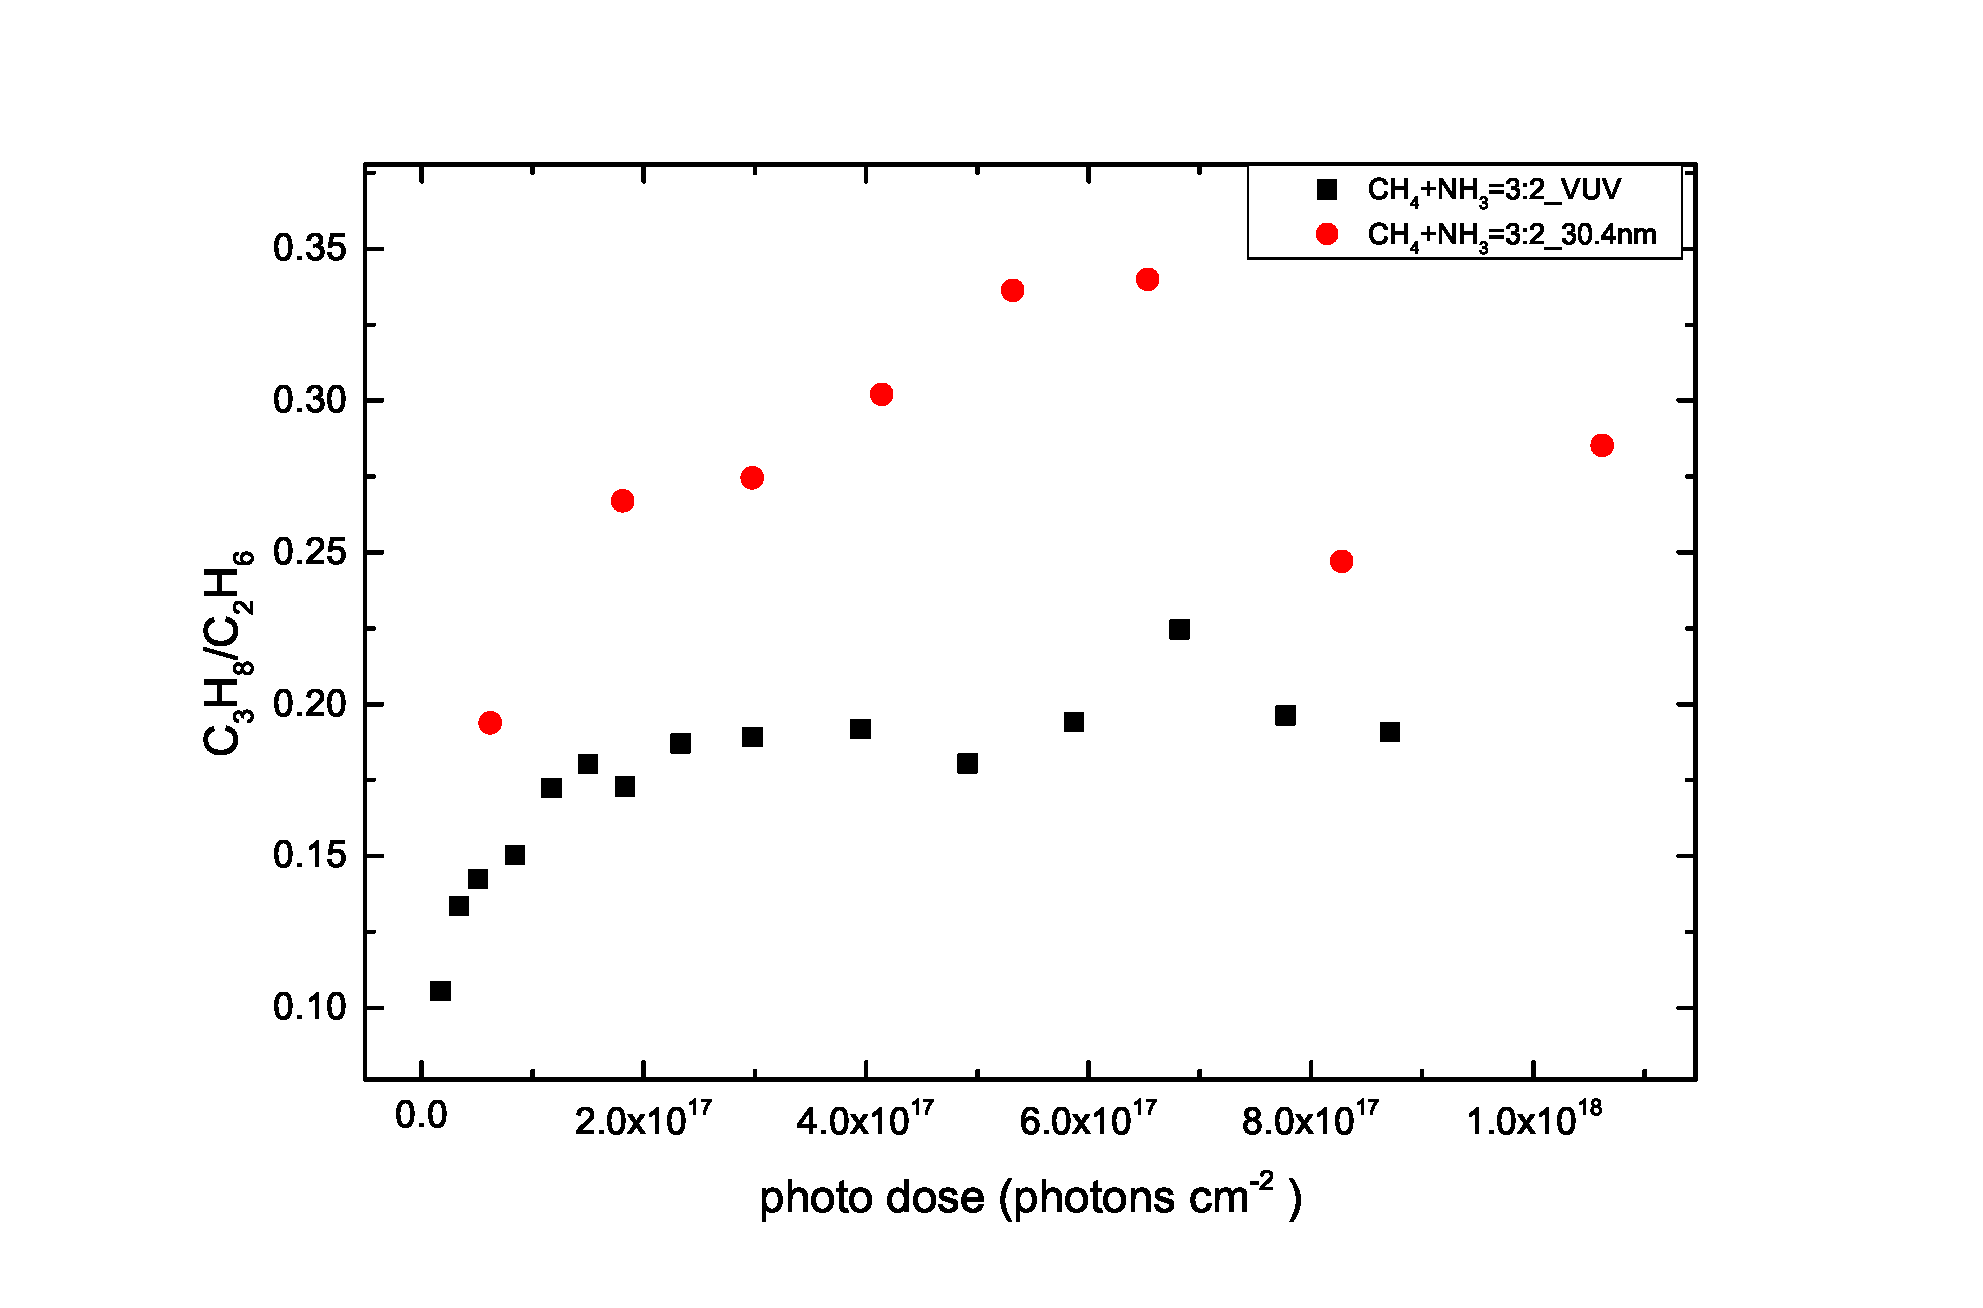
\includegraphics[width=\textwidth]{figures/chapter3/NSRRC_Lab_C3H8_C2H6.eps}
\caption{The column density of C$_3$H$_8$ divided by C$_2$H$_6$ accumulated when different configurations of CH$_4$ + NH$_3$ ice mixtures are irradiated by VUV and EUV photons}
\label{fig:NSRRC_Lab_C3H8_C2H6}
\end{figure}

Figure \ref{fig:NSRRC_Lab_C3H8_C2H6} shows the column density of C$_2$H$_6$ divided by C$_3$H$_8$ after CH$_4$ + NH$_3$ =3:2 ice mixtures are irradiated by VUV irradiation and He II monochromatic light.

From \ref{fig:NSRRC_Lab_C3H8_C2H6}, we may observe that more C$_3$H$_8$ is produced by 30.4nm photons than by VUV photons. Recall the formation mechanism of C$_3$H$_8$ (equation \ref{eq:C3H82}), CH$_2$ and C$_2$H$_4$ radicals are esccential in producing C$_3$H$_8$. This increase production in C$_3$H$_8$ may be caused by the increase in CH$_2$ radicals during fragmentation of CH$_4$. This result is similar to the findings of Gans et al. (2011), the ratio of CH$_2$ radicals increases from 0.3 to 0.48 when photon energy increases from 121.6 nm to 118.2 nm in their pulsed laser experiments.


\begin{figure}
\centering
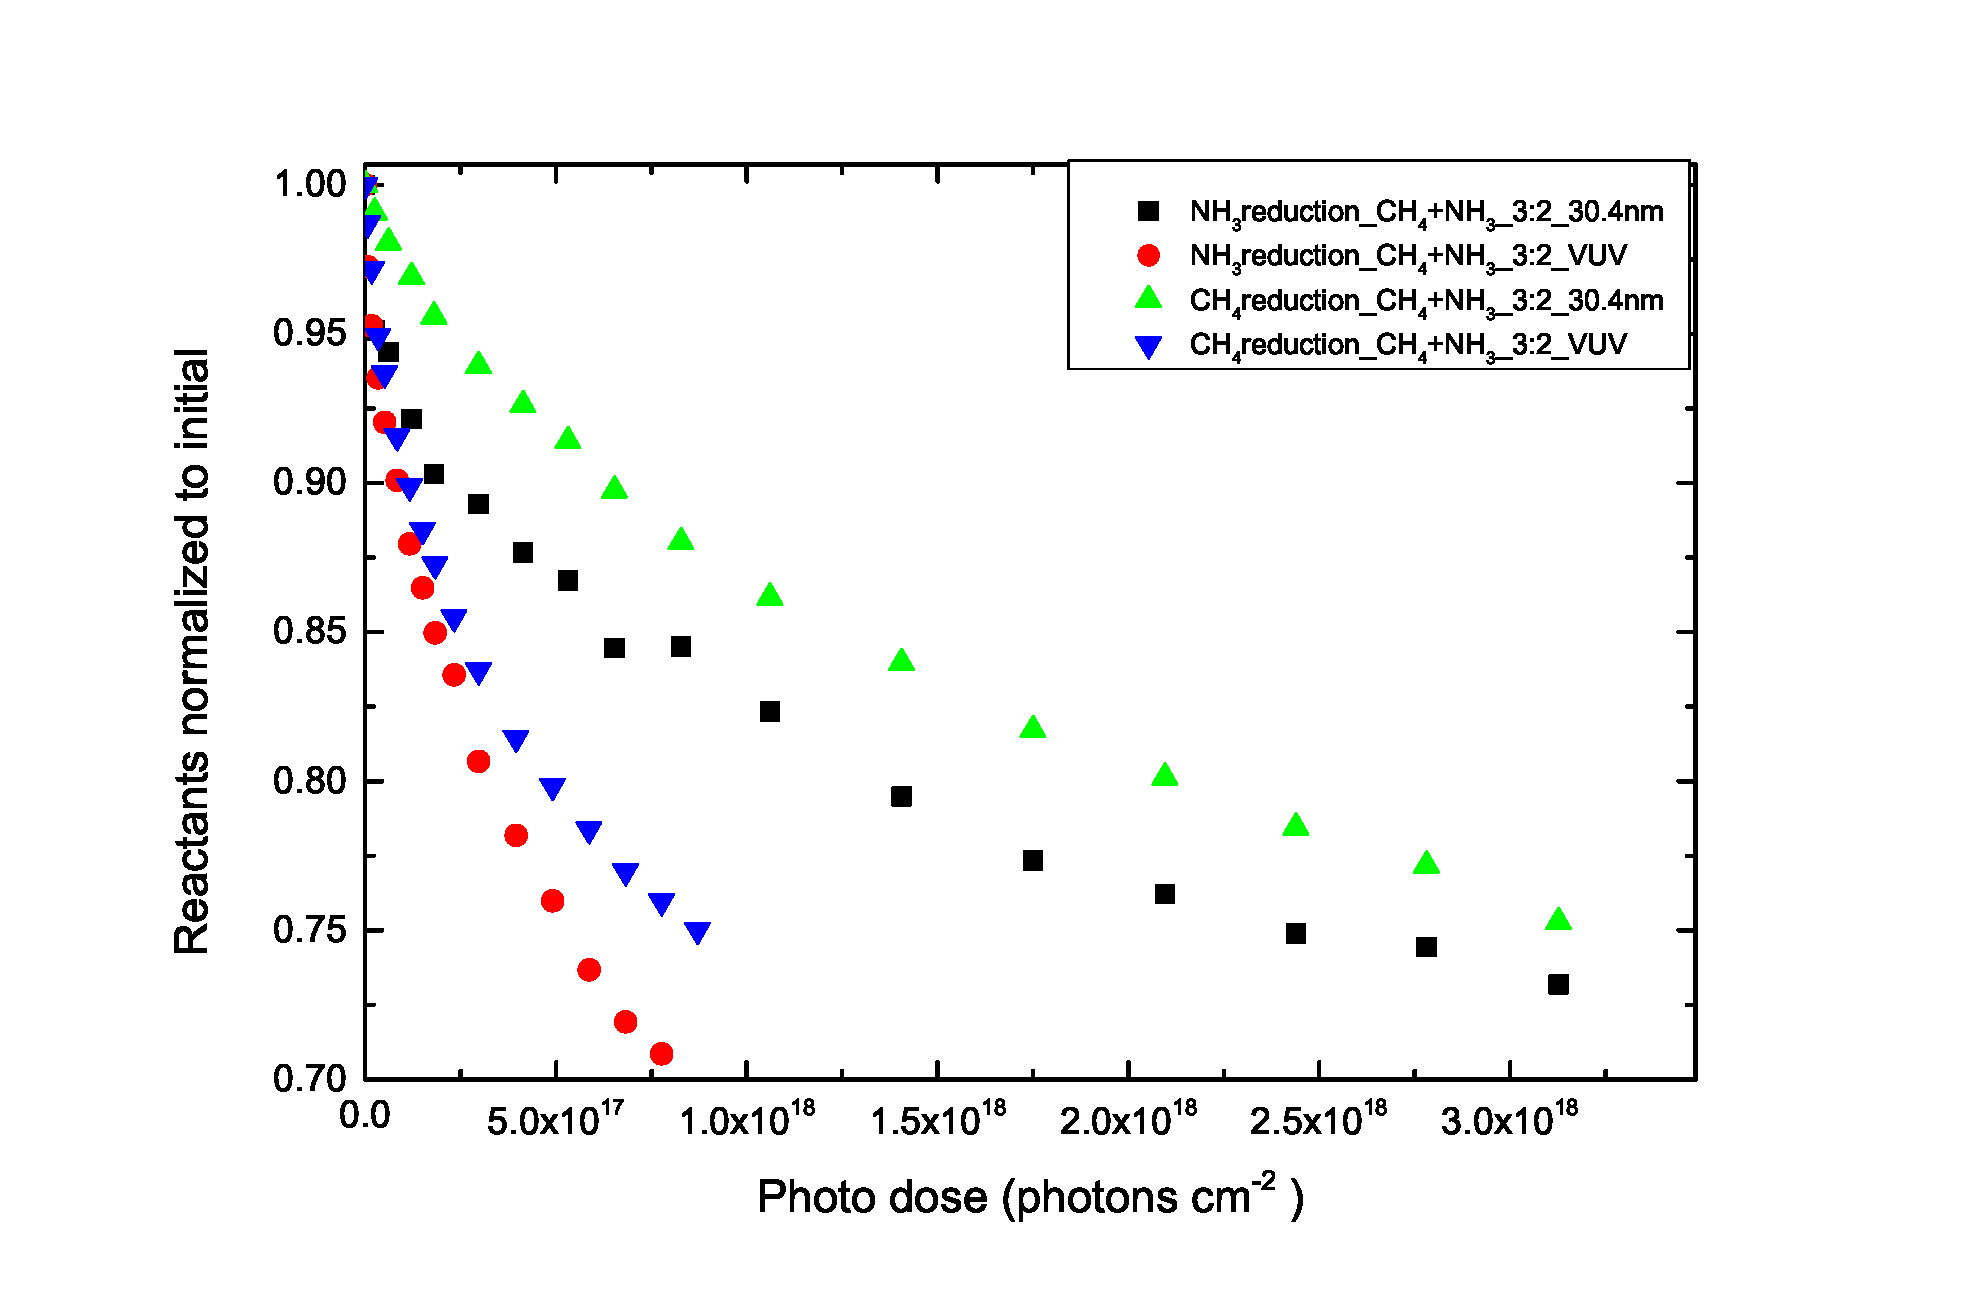
\includegraphics[width=\textwidth]{figures/chapter3/Reactants_normalized_to_initial.eps}
\caption{The normalized reduction of CH$_4$ and NH$_3$ in CH$_4$ + NH$_3$ ice mixtures irradiated by VUV and EUV photons}
\label{fig:normalized_reactants}
\end{figure}


Apart from C$_2$H$_6$ and C$_3$H$_8$, are there any difference in CN$^-$ production? Figure \ref{fig:CN_NSRRC} shows the accumulated column densities of CN$^-$ generated by irradiation of CH$_4$+NH$_3$ ice mixtures by MDHL and 30.4 nm monochromatic light. The fitting results are shown in Table 3.6. The rate constants forming CN$^-$ is 3.06 to 4.13 times larger in CH$_4$+NH$_3$ = 1:5 and 3:2 irradiated by MDHL than irradiated by 30.4 nm monochromatic light respectively. From figure \ref{normalized_reactants}, the CH$_4$ reduction in NSRRC is 6.06$\pm$0.07 times slower. With the rate constants of CN$^-$ only 3.06 to 4.13 times smaller, the 6 times slower in CH$_4$ reduction and 3 times slower in CN$^-$ formation give rise to a similarity of reduced NH$_3$ destruction cross-section and reduced rate in CN$^-$ production in EUV irradiation experiments. Therefore, we may conclude that the reduction in CN$^-$ formation rate by 30.4nm EUV irradiation is mainly due to the decreased NH$_3$ destruction cross-sections.

\begin{figure}
\centering
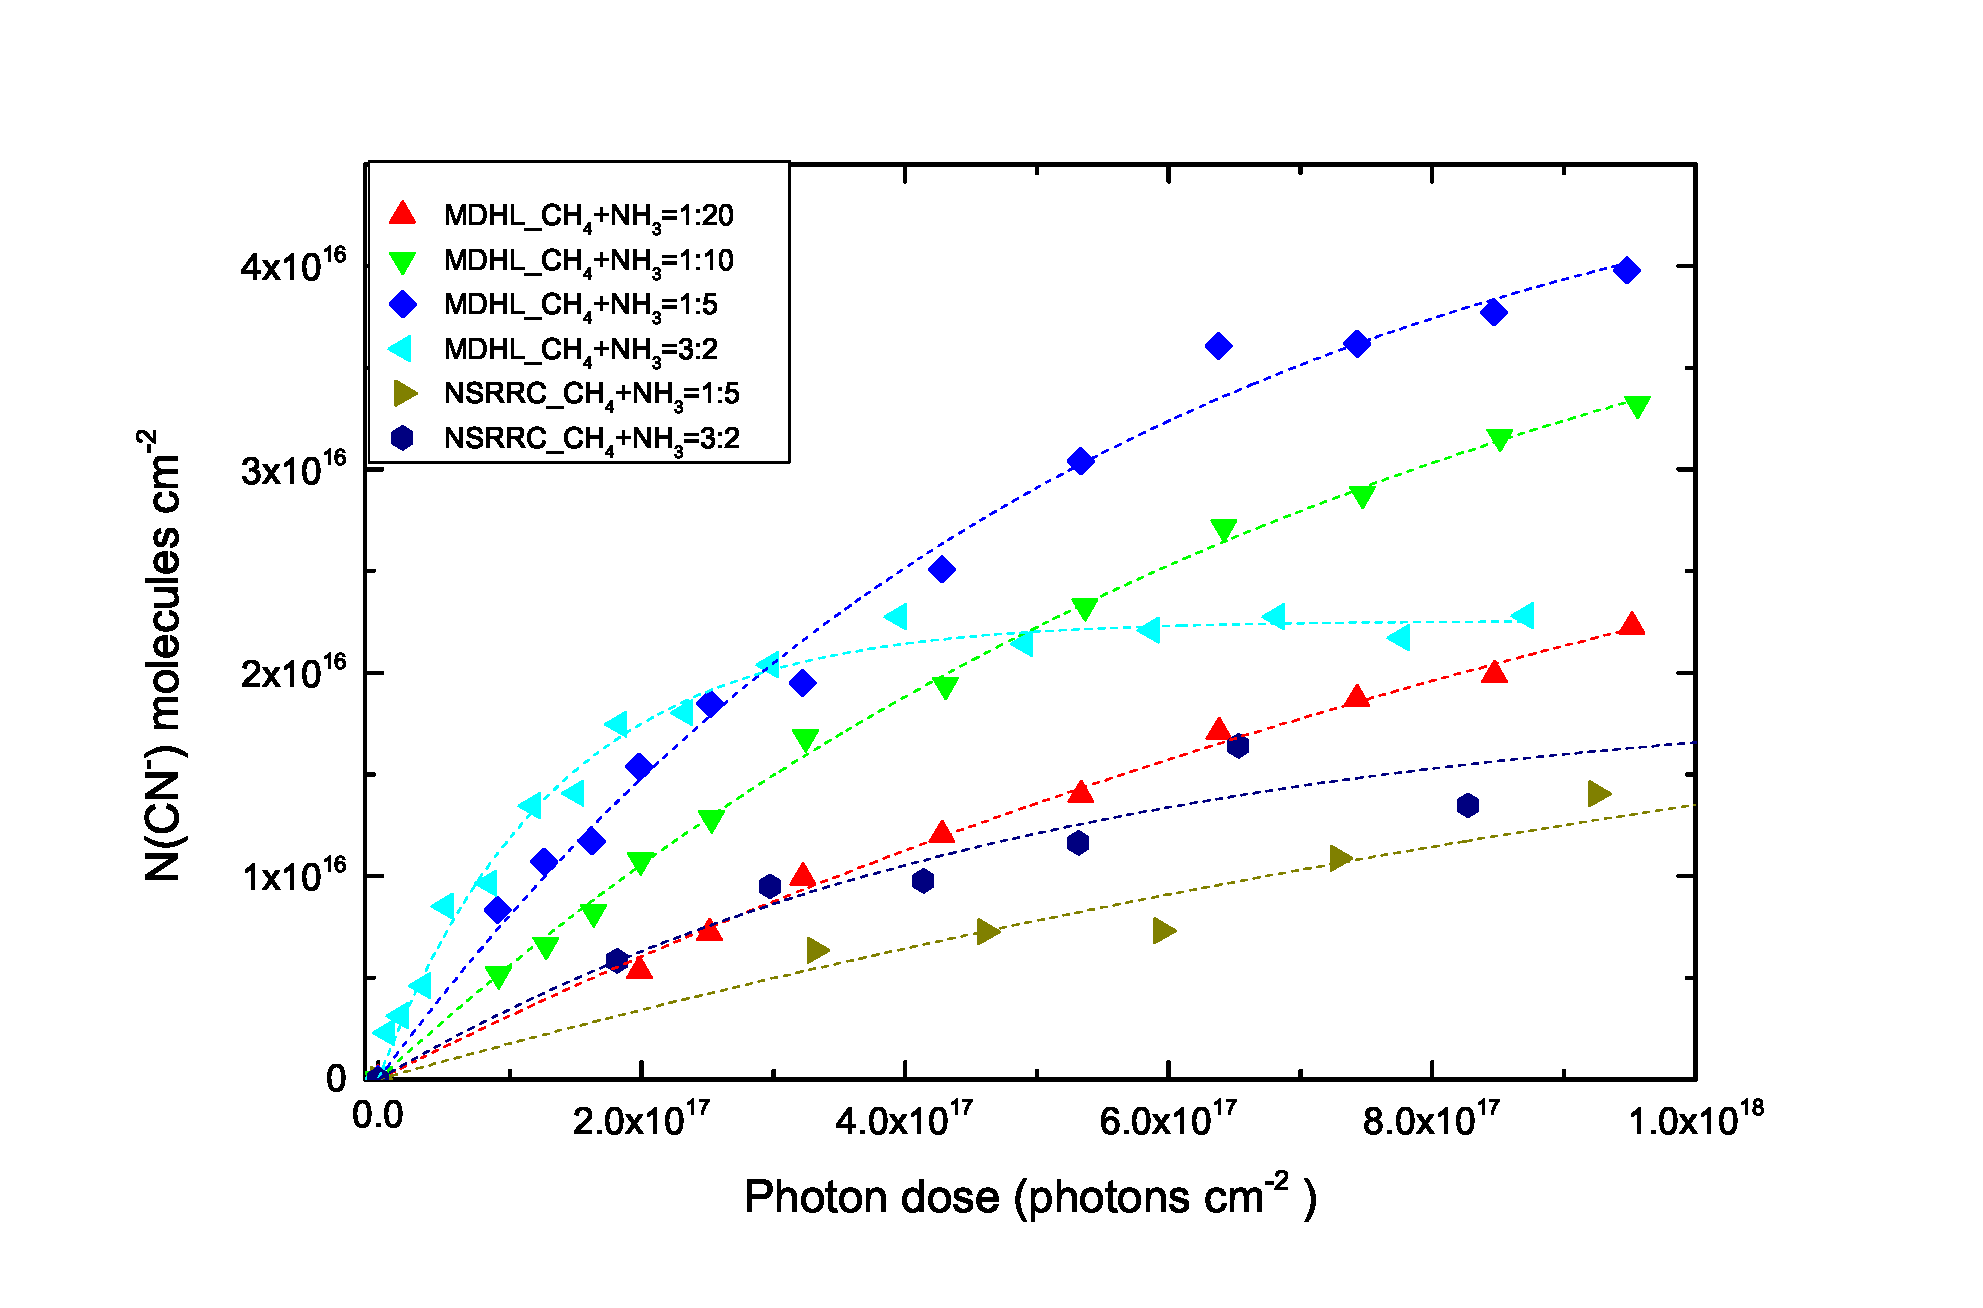
\includegraphics[width=\textwidth]{figures/chapter3/overall_CN_NSRRC.eps}
\caption{The column densities of CN$^-$ generated by irradiation of CH4+NH3 ice mixtures by MDHL and 30.4 nm monochromatic light.}
\label{fig:CN_NSRRC}
\end{figure}

\begin{table}[htbp]
\caption{The fitting results of CN$^-$ by equation \ref{eq:rate7}}
\label{tab:CNrate}
\begin{tabular}{ccccc}
\hline
\hline
Light source & Ratio of CH$_4$+NH$_3$ & A (x10$^{16}$ molecules cm$^{-2}$) & k$_1$ (x10$^{-18}$ photon$^{-1}$) & k$_2$ (photon$^{-1}$)\\
\hline
VUV & 1:5 & 4.61 $\pm$ 0.18 & 1.93 $\pm$ 0.19 & >1 \\
 & 3:2 & 2.24 $\pm$ 0.03 & 8.21 $\pm$ 0.70 & >1 \\
\hline
EUV & 1:5 & 2.89 $\pm$ 1.29 & 0.63 $\pm$ 0.37 & >1 \\
 & 3:2 & 2.24 $\pm$ 0.03 & 1.92 $\pm$ 1.99 & >1 \\
\hline
\end{tabular}
Fitting result of figure \ref{CN_NSRRC} with pseudo first order equation [CN$^-$]=$A(1-e^{-kx})$. These fitting results of MDHL experiments are an average of at least 2 experiments with the same circumstances. In the expression, A represents the column density when x, the photon dose, becomes infinitely large and k is the rate constant.\
\end{table}


\section{Residues}
The residues we studied are the accumulated residues onto the substrate. We do not understand are there any interaction between residues and the ice mixtures. However, we may know what is the change of residues when we change the ratio of the CH$_4$+NH$_3$ from CH$_4$ dominating to NH$_3$ dominating.  Figure \ref{residues} is a comparison of CH$_4$+NH$_3$ = 3:2 after VUV experiments, residues accumulated after EUV exposure of CH$_4$ + NH$_3$ = 3:2 ice mixtures and the plasma experiment done by Imanaka et al. (2004). The residues in ammonia dominated ice mixtures cannot be detected after consecutive experiments. There are no differences between EUV accumulated residues and VUV accumulated residues in CH$_4$+NH$_3$ = 3:2 ice mixtues. The main differences between plasma experiments of N$_2$+CH$_4$ (9:1) done at 2300 Pa. by Imanaka et al. (2004) and our experiments is the peaks located around 2090 cm$^{-1}$.

Why we use different initial reactants, replacing N$_2$ by NH$_3$ but we may get similar residues? The similarities during formation of atomic nitrogens when breaking N$_2$ bonds in nitrogen and NH bonds in ammonia give rise to this result. When photon energy is enough to break both NH bond and N$_2$ bond, similar experimental residues forms. Our results implies that the residues formed on Charon is similar to what we found on Titan, although their formation environments differs from gaseous phase with N$_2$ dominating to solid phase with NH$_3$.

After CH4+NH3 = 1:5, 1:10 and 1:20 experiments, we notice that two new bonds are formed. One at 1721 cm-1 and another at 1286 cm-1. These two peaks are due to MCT detector self-contamination. When we stopped adding liquid nitrogen, molecules stick onto MCT detector will be free out. They sticked onto our detector and hence produced these two peaks. Hence, we may conclude that the residues produced by CH4+NH3 with different ratios are the same.

\begin{figure}
\centering
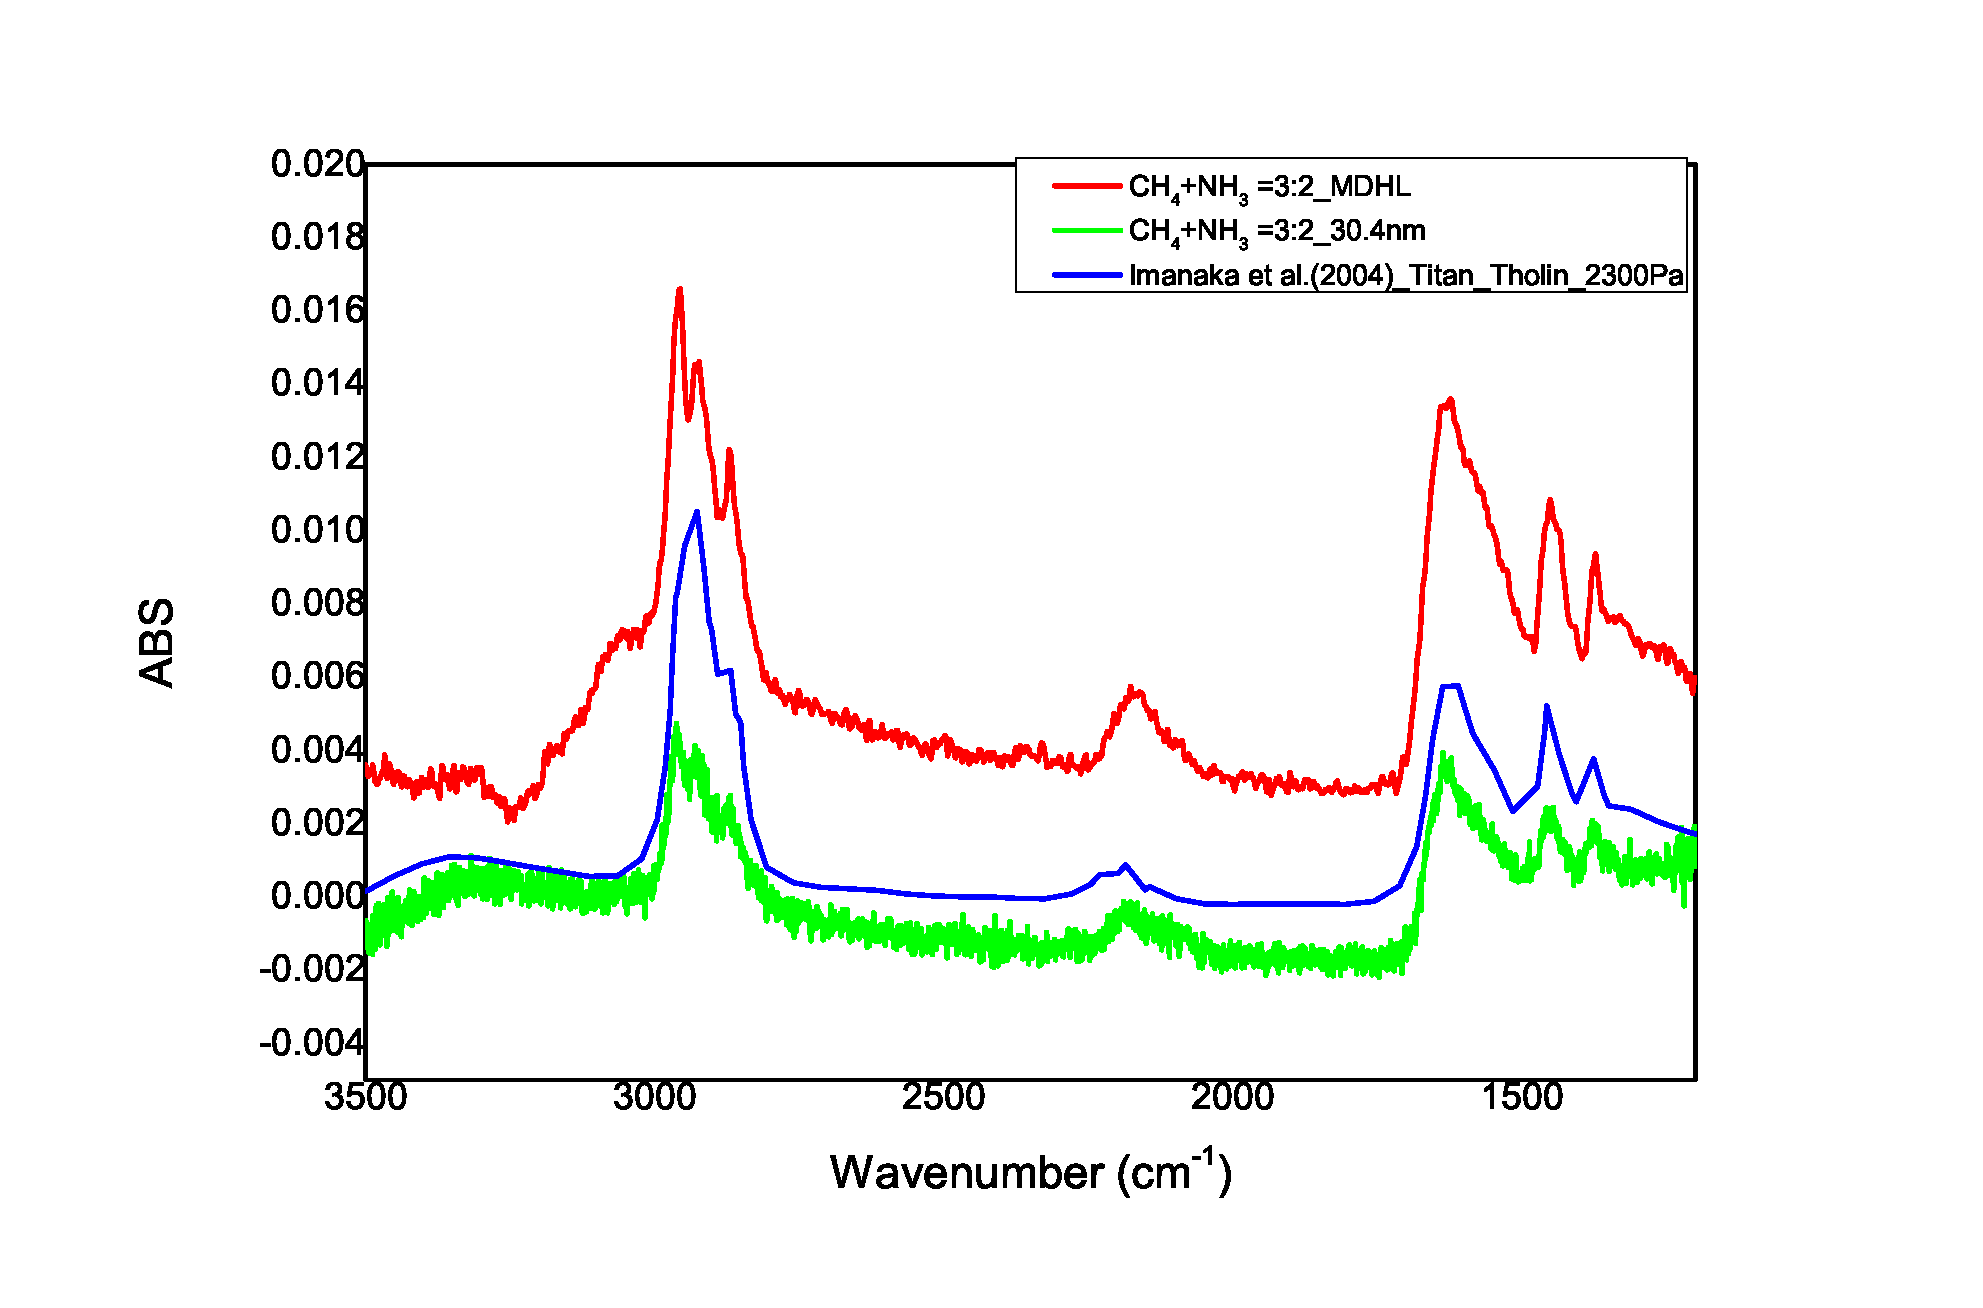
\includegraphics[width=\textwidth]{figures/chapter3/residue.eps}
\caption{The IR spectrum of residues in after CH$_4$+NH$_3$ = 3:2 experiments and the accumulate residues after MDHL experiments and NSRRC experiments.}
\label{fig:residues}
\end{figure}

